\documentclass[
    %draft, % Mit % kommentieren, um Bilder sichtbar zu machen und Links zu aktivieren
    pdftex,
    a4paper,
    oneside,
    parskip,
    numbers=noenddot,
    listof=totoc,
    bibliography=totoc,
    hyperfootnotes=false,
    english
]{scrreprt}
\setuptoc{toc}{totoc}

\newcommand{\thesistitle}{Identification of key information with topic analysis on large unstructured text data}
\newcommand{\thesistype}{B A C H E L O R  T H E S I S}
\newcommand{\thesistypedesc}{Department of Electrical Engineering and Computer Science \\
    University of Kassel}
\newcommand{\thesisauthorname}{Klara Maximiliane Gutekunst}
\newcommand{\thesisauthorhomestreet}{*** REMOVED ***}
\newcommand{\thesisauthorhometown}{34125 Kassel}
\newcommand{\thesisauthormatrikelnumber}{*** REMOVED ***}
\newcommand{\thesisauthoremail}{klara.gutekunst@student.uni-kassel.de}
\newcommand{\thesisdepartment}{Chair Intelligent Embedded Systems}
\newcommand{\thesisfirstreviewer}{Prof.\ Dr.\ rer.\ nat.\ Bernhard Sick}
\newcommand{\thesissecondreviewer}{Prof.\ Dr.\ Gerd Stumme}
\newcommand{\thesissupervisor}{Dr.\ Christian Gruhl}
\newcommand{\thesisdate}{\today}
\newcommand{\eigenfaces}{Eigenfaces}
\newcommand{\eigendocs}{Eigendocs}

% Select input encoding, usually utf8 is the best choice, on windows, \usepackage[latin1]{inputenc} maybe required
\usepackage[utf8]{inputenc}
\usepackage[T1]{fontenc}
\usepackage[english]{babel}
\usepackage{csquotes}
\usepackage{xcolor}

\MakeOuterQuote{"} % Damit ist es möglich, " " zu verwenden ohne Umlaut zu erzeugen
\defaulthyphenchar=127 % Dadurch werden auch Wörter mit Bindestrich getrennt, die schon Bindestriche enthalten.

% geometry
\usepackage[bindingoffset=1cm, left=2.5cm, right=2.5cm, top=2.5cm, bottom=2.5cm]{geometry}

% Headline
\usepackage{fancyhdr}
\pagestyle{fancy}
\renewcommand{\chaptermark}[1]{\markboth{\thechapter\ #1}{}}
\lhead{\leftmark} \rhead{\thepage}
\cfoot{}
\fancypagestyle{plain}{}

\RedeclareSectionCommand[beforeskip=1.5cm,afterskip=1cm]{chapter}

% Colors
\usepackage{color}
\usepackage{colortbl}

% Tables
\usepackage{tabularx}
\usepackage{multirow}
\setlength{\tabcolsep}{4pt}

% Drawing graphs etc.
\usepackage{pgf}
\usepackage{tikz}
\usetikzlibrary{arrows,automata}

% Footnotes
\usepackage{footmisc}
\usepackage{xspace}
\newcommand{\sic}{[\acs{sic}]\xspace}

% math
\usepackage{amsmath}
\usepackage{amssymb}

\usepackage{siunitx}

% lists
\usepackage{paralist}

% Figures
\usepackage{graphicx, wrapfig}

% Hyperlinks
\usepackage[hyphens]{url}
\usepackage{hyperref}
\hypersetup{colorlinks, citecolor=black, linkcolor=black, urlcolor=black}

% Minted
\usepackage[chapter]{minted}
%\usemintedstyle{xcode}
\setminted{frame=single,tabsize=2,linenos,autogobble}

\newmintinline[code]{text}{breaklines}

\newminted[mdcodeblock]{md}{autogobble,frame=none,linenos=false,breaklines}

% list of abbreviations
\usepackage[printonlyused]{acronym}

% Set line pitch
\usepackage{setspace}
\onehalfspacing              % anderthalbzeilig (oder auch \doublespace)

%fancyBox
%\usepackage{fancybox}

% Layout corrections (Schusterjungen)
\clubpenalty = 10000
% Layout corrections (Hurenkinder)
\widowpenalty = 10000
\displaywidowpenalty = 10000

% Figures
\usepackage{caption}
\usepackage[hypcap=true,labelformat=simple]{subcaption}
\renewcommand{\thesubfigure}{(\alph{subfigure})}
\usepackage[inkscapelatex=false]{svg}

% Tables
\usepackage{booktabs}
%\usepackage[table,xcdraw]{xcolor}

% enumerate
\usepackage{enumitem}

% Bibliography
\usepackage[square,numbers]{natbib}
\bibliographystyle{plainnat} % or plainnat abbrvnat unsrtnat

% Frequently used column types
\newcolumntype{C}[1]{>{\centering\arraybackslash}p{#1}} % centering column type with fixed width
\newcolumntype{R}[1]{>{\raggedleft\arraybackslash}p{#1}} % right aligned column type with fixed width
\newcolumntype{L}[1]{>{\raggedright\arraybackslash}p{#1}} % left aligned column type with fixed width

% Shortcuts for referencing floats:
\newcommand{\fig}[1]{\figurename~\ref{#1}} %shortcut for a figure reference
\newcommand{\tab}[1]{Table~\ref{#1}} %shortcut for a table reference
\newcommand{\eq}[1]{(\ref{#1})} %shortcut for an equation reference
\newcommand{\lst}[1]{Listing~\ref{#1}} %shortcut for a listing reference
\newcommand{\sect}[1]{Section~\ref{#1}} %shortcut for a Section reference

% Shortcut for terms
\newcommand{\databaseName}{Elasticsearch}



\begin{document}

    \pagenumbering{roman}

    \begin{titlepage}
	% Select font without serifs
	\sffamily

	% Logo
	\begin{tabularx}{\textwidth}{@{}l@{}>{\raggedleft\arraybackslash}X@{}r@{}}
		\multirow{2}{*}{
\includegraphics[width=6.8cm]{images/Logo_UniKassel}} &
		\raisebox{-1mm}{\small{Department of Electrical Engineering and Computer Science}} \\
		&\raisebox{-1mm}{\small{\thesisdepartment}} &
	\end{tabularx}

	\vspace{2.5cm}

	\begin{center}
		% Title and subtitle
		\huge{\thesistitle}

		\vspace{3cm}

		\renewcommand{\baselinestretch}{1.3}
		\Large{\thesistype}

		\large
		\thesistypedesc
	\end{center}

	\vspace{1.5cm}
	\renewcommand{\baselinestretch}{1}
	\begin{table}[htpb]
		\centering
		\begin{tabular}{ll}
			\\
			Author Name: & \thesisauthorname \\
			Address: & \thesisauthorhomestreet \\
			& \thesisauthorhometown \\
			\\
			Matriculation number: & \thesisauthormatrikelnumber \\
			E-Mail: & \thesisauthoremail \\
			\\
			Department: & \thesisdepartment \\
			\\
			Examining board 1: & \thesisfirstreviewer \\
			Examining board 2: & \thesissecondreviewer \\
			\\
			Supervisor: & \thesissupervisor \\
			\\
			Date: & \thesisdate \\
		\end{tabular}
	\end{table}

	% font with serifs
	\rmfamily
\end{titlepage}

    \chapter*{Abstract}

% Inhaltsverzeichnis und Kopfzeile
\addcontentsline{toc}{chapter}{Abstract}
% left paranthese for side header of even numbered page, right one for odd numbered page
\markboth{Abstract}{Abstract}


Finding relevant documents and connections between multiple ones becomes significantly more difficult due to the sheer amount of documents available.
Reviewing all documents in the course of the exploration of the data is no longer an option and thus, exploratory data analysis (EDA) is very important.

Institutes, such as the (German) tax offices have access to leak data containing huge amounts of documents and valuable information yet to be extracted.
However, these institutes, companies and individuals do not have sufficient resources to explore individual documents in order to find a specific one or to identify the key topics of them.
Hence, computational means, such as text mining, may facilitate the situation.
Text mining is used to automatically extract knowledge or information from unstructured text data.
Text mining is a discipline of data mining.

In this case, the starting point is a large text corpus.
Since the leaks of (German) tax offices are restricted due to confidentiality reasons, free and online accessible data for instance from Wikipedia or Twitter, containing multiple documents of unknown and diverse content will be used for this thesis.

In order to explore texts methods of topic modelling may be used.
In this thesis, these methods are first identified via literature research and applied after.
Potentially applicable methods include LDA in combination with visualisation via Wordclouds or BERTopic.


The topics to be identified can be groups of words which appear more often than the average or groups of similar documents.
Hence, a topic is not always the defined topic in terms of content, but sometimes a statistical phenomenon.
Since different methods will probably define different topics, as they work and define the meaning of 'topic' differently, their results will be compared and evaluated on the dataset.

Besides literature research, application and evaluation of the methods identified, certain preprocessing methods will probably prove to be eminent to successful work with unstructured text data.
These methods could include chunking (separating texts into equally sized segments), lemmatization (eg. faster to fast), conversion to small letters, and Part of Speech (POS) for analysis and potential exclusion of certain named entities (NER) and stop-word-lists.

First research showed that Natural Language Toolkit (NLTK) may be a library of interest in this context.

    \tableofcontents

    \chapter*{List of abbreviations}
\markboth{List of abbreviations}{List of abbreviations}

\begin{acronym}[XXXXXXXXX]
    \acro{acid}[ACID]{Atomicity, Consistency, Isolation, Durability}
    \acro{ae}[AE]{Autoencoder}
    \acro{annoy}[Annoy]{Approximate Nearest Neighbours Oh Yeah}
    \acro{api}[API]{Application Programming Interface}
    \acro{bertopic}[BERTopic]{BERT Topic Model}
    \acro{bert}[BERT]{Bidirectional Encoder Representations from Transformers}
    \acro{bilstm}[BiLSTM]{Bi-directional Long Short-Term Memory}
    \acro{bow}[BoW]{Bag of Words}
    \acro{cbow}[CBOW]{Continuous-Bag-of-Words}
    \acro{cpu}[CPU]{Central Processing Unit}
    \acro{css}[CSS]{Cascading Style Sheet}
    \acro{csv}[CSV]{Comma Separated Values}
    \acro{d2v}[Doc2Vec]{Document to Vector}
    \acro{dan}[DAN]{Deep Averaging Network}
    \acro{dbscan}[DBSCAN]{Density-Based Spatial Clustering of Applications with Noise}
    \acro{dnn}[DNN]{Deep Neural Network}
    \acro{etc}[etc.]{et cetera}    
    \acro{gb}[GB]{Gigabyte}
    \acro{glove}[GloVe]{Global Vectors}
    \acro{gpu}[GPU]{Graphics Processing Unit}
    \acro{hdbscan}[HDBSCAN]{Hierarchical DBSCAN}
    \acro{hnsw}[HNSW]{Hierarchical Navigable Small World}
    \acro{html}[HTML]{Hypertext Markup Language}
    \acro{http}[HTTP]{Hypertext Transfer Protocol}
    \acro{idf}[IDF]{Inverse Document Frequency}
    \acro{ies}[IES]{Intelligent Embedded Systems}
    \acro{ir}[IR]{Information Retrieval}
    \acro{json}[JSON]{JavaScript Object Notation}
    \acro{kl}[KL]{Karhonen-Loéve}
    \acro{knn}[kNN]{k-nearest neighbor}
    \acro{lda}[LDA]{Latent Dirichlet Allocation}
    \acro{lstm}[LSTM]{Long Short-Term Memory}
    \acro{ml}[ML]{Machine Learning}
    \acro{nli}[NLI]{Natural Language Inference}
    \acro{nlp}[NLP]{Natural Language Processing}
    \acro{nltk}[NLTK]{Natural Language Toolkit}
    \acro{nn}[NN]{Neural Network}
    \acro{nosql}[NoSQL]{Not only SQL}
    \acro{optics}[OPTICS]{Ordering Points To Identify the Clustering Structure}
    \acro{pca}[PCA]{Principal Component Analysis}
    \acro{pdf}[PDF]{Portable Document Format}
    \acro{pkl}[PKL]{Pickle}
    \acro{png}[PNG]{Portable Network Graphics}
    \acro{pvdbow}[PV-DBOW]{Distributed Bag of Words}
    \acro{pvdm}[PVDM]{Paragraph Vector Distributed Memory}
    \acro{rmse}[RMSE]{Root Mean Square Error}
    \acro{rnn}[RNN]{Recurrent Neural Network}
    \acro{rq}[RQ]{Research Question}
    \acro{rsme}[RSME]{Root Mean Square Error}
    \acro{sbert}[SBERT]{Sentence-BERT}
    \acro{snli}[SNLI]{Stanford Natural Language Inference}
    \acro{sql}[SQL]{Structured Query Language}
    \acro{ssh}[SSH]{Secure Socket Shell}
    \acro{svd}[SVD]{Singular value decomposition}
    \acro{svm}[SVM]{Support Vector Machine}
    \acro{t2v}[Top2Vec]{Topic to Vector}
    \acro{tfidf}[TF-IDF]{Term Frequency - Inverse Document Frequency}
    \acro{tf}[TF]{Term Frequency}
    \acro{ui}[UI]{User Interface}
    \acro{umap}[UMAP]{Uniform Manifold Approximation and Projection}
    \acro{url}[URL]{Uniform Resource Locator}
    \acro{use}[USE]{Universal Sentence Encoder}
    \acro{vscode}[VSCode]{Visual Studio Code}
    \acro{vsm}[VSM]{Vector Space Model}
    \acro{w2v}[Word2Vec]{Word to Vector}
    \acro{wmd}[WMD]{Word Mover's Distance}
    \acro{xml}[XML]{Extensible Markup Language}
\end{acronym}


    \pagebreak
    \pagenumbering{arabic}

    % Hier weitere Kapitel einfügen
    \chapter{Introduction}\label{ch:introduction}

\section{Motivation/ Objective}\label{sec:motivation}
Zielsetzung


\section{Related work}\label{sec:related-work}


\section{Research Questions}\label{sec:research-questions}

list of research questions
\subsection[\acs{rq}1]{\ac{rq}1: Question 1?}\label{subsec:rq1}
explanation of \ac{rq}1


\section{Structure of the Thesis}\label{sec:structure-of-the-thesis}
    \chapter{Related work}\label{sec:related-work}
    \chapter{Fundamentals/ State of the art}\label{ch:methodology}

\cite{InformationRetrieval1999}

Basic concepts, methods used, etc.



\section{Preprocessing}\label{sec:preprocessing}


\subsection{Tokenization/ Chunking}\label{subsec:tokenization}

\textit{Tokenization} is the process of splitting a text into smaller pieces, so-called \textit{tokens}.
Tokens can be words and punctuation marks \cite{nlp-book2009}.
However, the definition of a token depends on the application.
For instance, certain tokenization implementations may identify tokens as subsequent series of non-whitespace characters omitting all numbers and punctuation marks \cite{IR2011}.

\textit{Chunking} is the process of splitting a text into smaller pieces, so-called \textit{chunks}.
A chunk is a sequence of tokens, e.g. words, in a text \cite{nlp-book2009}.
Chunks do not overlap.
According to \citeauthor{nlp-book2009}, chunkers produce their pieces by following a set of rules, e.g., grammar rules.

\subsection{Stemming}\label{subsec:stemming}

According to \citeauthor{nlp-book2009}, \textit{stemming} is the process of striping off any affixes, i.e. prefixes and suffixes \cite{IR2011}, from a word and returning the stem.
Different types of stemmers are better suited for certain applications than others.
Hence, the choice of the stemmer depends on the application.
For instance, the \textit{Porter Stemmer} performs well when indexing texts and for text search using alternative forms, 
i.e. adding and omitting affixes, of words \cite{nlp-book2009}.
The \textit{Porter Stemmer} is a rule-based stemmer, i.e. it applies a set of rules to a word to produce the stem and thus, does not use a dictionary \cite{IR2011}.

\subsection{Lemmatization}\label{subsec:lemmatization}

By ensuring the resulting stem is a valid word, the process of stemming is called \textit{lemmatization} \cite{nlp-book2009}.
Some implementations of lemmatizers only stem words if the result is in its dictionary.
Since lemmatizers validate the result prior to returning it, they are usually slower than stemmers \cite{nlp-book2009}.


\subsection{Stop-Word-Removal}\label{subsec:stop-word-removal}

Omitting words that are not relevant to the context of the text is called \textit{stop-word-removal}.
Stop words not only depend on the domain but also on the language \cite{IR2011}.
Possibly, domain-specific stop-word lists are used to remove words that are not relevant to the context of the text \cite{IR2011}.



\subsection{Lower case}\label{subsec:lower-case}

Words with capital letters are converted to lowercase.



\section{Similarity Measurement}\label{sec:similarity-measurement}

Since embeddings represent texts as vectors, they not only facilitate human interpretability of relationships between texts using 
the text's respective point in a $N$-dimensional space, but also enable the use of similarity measures to quantify the similarity between texts.
A similarity measure defines a metric to quantify the similarity between two texts \cite{IR2011, euclidean_l2_norm2015}.

There are several similarity measures, such as the dot product quantifying the number of shared tokens of two texts, 
the (soft) cosine similarity, which is the normalized dot product and calculates the angle between two vectors, 
and many more \cite{IR2011, euclidean_l2_norm2015, HfsentTrans2019}.
The following section describes a few of the metrics usable for similarity measurement.


\subsection{Euclidian distance}\label{subsec:euclidian-distance}

The \textit{euclidian distance} is a distance measure.
In order to measure the distance between two points in a $N$-dimensional space, 
the root of the sum of squared distances between the respective values of every dimension is calculated.
The distance function Euclidean (L2) norm is given in \autoref{eq:euclidian-distance} from \cite{euclidean_l2_norm2015}.
The points $x_1, x_2$ correspond to objects $d_1, d_2$.

\begin{equation}
    d_E(x_1,x_2) = \sqrt{\sum_{i=1}^{N}(x_1\left[ i \right] - x_2\left[ i \right])^2}
    \label{eq:euclidian-distance}
\end{equation}


\subsection{Cosine Similarity}\label{subsec:cosine-similarity}

In the traditional bag-of-words approach the texts are represented as vectors of \ac{tfidf} coefficients \cite{soft_cosine2017}.
Without further processing, the vector is of size $N$, $N$ being the number of different words of the texts \cite{soft_cosine2017}.
Hence, a vector represents its corresponding text in a $N$-dimensional space.
This space is called \ac{vsm} \cite{soft_cosine2014}.

The similarity between two texts is measured by the cosine of the angle between their respective vectors \cite{soft_cosine2014}.
The cosine similarity is defined in \autoref{eq:cosine-similarity} from \cite{soft_cosine2014}.
$a \cdot b = \sum_{i=1}^{N}a_{i}b_{i}$ is the dot-product.
The dot-product is normalized with $\left\| x \right\| = \sqrt{x \cdot x}$ to unit Euclidean length \cite{soft_cosine2014}.
The cosine similarity is a value between $0$ and $1$ for positive values \cite{soft_cosine2014}.
According to \citeauthor{soft_cosine2014}, the formula has a time and space complexity of $O(N)$ for a pair of $N$-dimensional vectors.

\begin{equation}
    cosine(a,b) = \frac{a \cdot b}{\left\| a \right\| \times \left\| b \right\|} = \frac{\sum_{i=1}^{N}a_{i}b_{i}}{\sqrt{\sum_{i=1}^{N}{a}^2_{i}}\sqrt{\sum_{i=1}^{N}{b}^2_{i}}}
    \label{eq:cosine-similarity}
\end{equation}

The formula \autoref{eq:cosine-similarity} assumes that the vectors, which span the \ac{vsm} are orthogonal and thus, 
completely independent \cite{soft_cosine2014}.
However, in practical applications, this often is not the case \cite{soft_cosine2014}.


\subsection{Soft Cosine Similarity}\label{subsec:soft-cosine-similarity}

This similarity measure not only evaluates whether two texts consist of the same words but 
also takes into account the semantic (word-level) similarity or lexical relation of different words of the texts \cite{soft_cosine2017}.
Hence, it improves the shortcomings of the traditional cosine similarity measure, 
which assumes the tokens of the vocabulary are completely independent of each other \cite{soft_cosine2014}.

According to \citeauthor{soft_cosine2014}, in order to model this additional information, more dimensions are added to the \ac{vsm}.
These dimensions can be obtained, for instance, by multiplying the mean of two features of one vector with the similarity between them \cite{soft_cosine2014}.
The similarity can be calculated by using Levenshtein distance for e.g., n-grams, i.e. the number of operations necessary to convert one string into another, 
or using a dictionary of synonyms \cite{soft_cosine2014}.

Since this approach no longer assumes that different words are independent of each other, 
the basis vectors which span the \ac{vsm} are no longer orthogonal \cite{soft_cosine2014}.
The formula for the soft cosine similarity is defined in \autoref{eq:soft-cosine-similarity} from \cite{soft_cosine2014}.
The similarity $s_{ij}$ between the $i$-th and $j$-th basis vector is obtained using a similarity measure, such as synonymy \cite{soft_cosine2014}.

\begin{equation}
    soft\_cosine(a,b) = \frac{\sum_{i=1}^{N}\sum_{j=1}^{N}s_{ij}a_{i}b_{j}}{\sqrt{\sum_{i=1}^{N}\sum_{j=1}^{N}s_{ij}a_{i}a_{j}}\sqrt{\sum_{i=1}^{N}\sum_{j=1}^{N}s_{ij}b_{i}b_{j}}}
    \label{eq:soft-cosine-similarity}
\end{equation}

According to \citeauthor{soft_cosine2017}, the similarity between two texts is non-zero as soon as they share related words \cite{soft_cosine2017}.
If there is no similarity between different features, 
the soft cosine similarity from \autoref{eq:soft-cosine-similarity} is equal to the cosine similarity from \autoref{eq:cosine-similarity}.
The time and space complexity of the soft cosine similarity is $O(N^2)$ \cite{soft_cosine2014}.

In order to reduce the complexity, \citeauthor{soft_cosine2014} propose to use a sparse similarity matrix which only stores $s_{ij} > t$, 
$t$ being a threshold \cite{soft_cosine2014}.


\section{Embeddings}\label{sec:embeddings}

Usually, \ac{ml} techniques embeddings, such as K-Means, require the text input data to be converted to embeddings \cite{SentRep2014}.
Embeddings are numerical representations of words, sentences or texts.
They can be used to present the textual data as real-valued vectors in a \ac{vsm}.
\acp{vsm} are commonly used due to their conceptual simplicity and because spatial proximity serves as a metaphor for semantic proximity 
\cite{tfidf2008, UniversalSentEnc2018, HfsentTrans2019, Top2Vec2020}.
Representations in a vector space can improve the performance in \ac{nlp} tasks \cite{SkipGram2013}.
According to \citeauthor{tfidf2008}, when representing text the first step is indexing, i.e. assigning indexing terms to the document.
The second task is to assign weights to the terms which correspond to the importance of the term in the document.
The weights assigned depend on the method and the assumptions of the model chosen to carry out the assignments.

The following section outlines a selection of embeddings.
Let a corpus of documents be denoted $D= \left\{d_1, d_2, ..., d_M  \right\}$, the number of documents in the dataset $M = \left\| D \right\|$,
a sequence of terms $w_{ij}$ or so-called document $d_i = \left\{w_{i1}, w_{i2}, ..., d_{iV}  \right\}$, $V$ being the length of the vocabulary, 
i.e. set of distinct words, of the corpus of documents \cite{clusteringDocs2020}.


\subsection{\ac{tfidf}}\label{subsec:tfidf}

\ac{tfidf} provides a numerical representation of a word in a document \cite{clusteringDocs2020}.
It considers the frequency of a word in a document and the frequency of a word in the whole corpus. 

\ac{tfidf} is calculated as displayed in \autoref{eq:tfidf-formula} from \cite{clusteringDocs2020} and exemplatory in \autoref{fig:tfidf-calculation}.
\ac{tf} is computed using $TF(w_{ij}, d_i) = f_{w_{ij}, d_i}$, whereas the \ac{idf} is computed using $IDF(w_{ij}, D) = \log_2\frac{M}{M_{ij}}$, 
$M_{ij}$ being the number of documents the term $w_{ij}$ appears in.
\ac{idf} measures the importance of a term $w_{ij}$ in the corpus of documents $D$.
The underlying assumption of \ac{idf} is that a term's importance to the data corpus is inversely proportional to its occurrence frequency \cite{tfidf2008}.
In other words: Terms which appear in many documents are not as important and thus, weighted less than document-specific terms. 

\begin{equation}
    TFIDF(w_{ij}, d_i, D) = TF(w_{ij}, d_i) \cdot IDF(w_{ij}, D)
    \label{eq:tfidf-formula}
\end{equation}


\begin{figure}[htp] % htp = hier (h), top (t), oder auf einer eigenen Seite (p).
    \centering
    \includesvg[width=0.7\textwidth]{images/embeddings/tfidf/tfidf.svg}
    \caption{
        Example of calculation of \ac{tfidf} parts: 
        \ac{tf} only considers the documents of interest while 
        \ac{idf} incorporates the importance of the word with respect to the whole dataset.
    }
    \label{fig:tfidf-calculation}
\end{figure}

\textcolor{red}{TODO: svg about tfidf}

According to \citeauthor{tfidf2008}, the computation complexity of \ac{tfidf} embeddings is $O(V \cdot M)$
The \ac{tfidf} more has several drawbacks \cite{clusteringDocs2020,tfidf2008}:
\begin{itemize}
    \item \ac{tfidf} does not consider semantic similarities between words.
    \item \ac{tfidf} does not consider the order of words in a document.
    \item \ac{tfidf} often produces high dimensional representations which have to be postprocessed to reduce their dimensionality, e.g., using \ac{pca}.
    \item The embeddings are not derived from a mathematical model of term distribution and may be criticised as not well reasoned.
\end{itemize}

\subsection{\ac{d2v}}\label{subsec:doc2vec}

Another term used for \ac{d2v} is \textit{Paragraph Vector} \cite{clusteringDocs2020}.
\ac{d2v} addresses the problems of \ac{tfidf} by encoding texts as $n-$dimensional vectors learnt using the words' context \cite{clusteringDocs2020}.
Hence, it preserves semantic similarities between words.
According to \citeauthor{clusteringDocs2020}, \ac{d2v} learns continuous distributed vector representations for pieces of the text.
The model handles inputs of different dimensions.

\ac{d2v} is an adaption of the \ac{w2v} model, which maps words into a \ac{vsm} under consideration of their semantic similarities \cite{clusteringDocs2020}.
The underlying hypothesis of both approaches is that words appearing in similar contexts are semantically similar \cite{clusteringDocs2020}.
The \ac{w2v} embedding is obtained using a \ac{nn} \cite{clusteringDocs2020}.
The \ac{nn} is shallow, i.e. has only one hidden layer.
This hidden layer creates the embedding of input data.
There are two approach as to how design the architecture of the \ac{nn}:
\begin{itemize}
    \item \ac{cbow}: 
        Predicts a word given a context
    \item Skip-Gram: 
        Predicts the context given a word.
\end{itemize}

The \ac{pvdm} extends the \ac{cbow} to work on corpus of documents instead of set of words \cite{clusteringDocs2020}:
As usual, vectors representing the words are obtained using the \ac{cbow} model.
Each document is mapped to a vector using an additional document-to-vector matrix.
The document vector is concatenated to the word vectors.
The resulting vector is used to predict the central word.
\textcolor{red}{prediction, loss function? B. in paper}

% paper widerspricht sich
%According to \citeauthor{clusteringDocs2020}, the \ac{doc2vec} model's performance is influenced quality of the preprocessing.
%If for instance, the stemmer assigns words with different meaning to the same root, there is a degradation in performance.


\cite{SentRep2014}
two flavor of doc2vec: PV-DM and PV-DBOW (https://thinkinfi.com/simple-doc2vec-explained/)
\cite{SkipGram2013}

\subsection{\ac{use}}\label{subsec:univ-sent-encoder}

\citeauthor{UniversalSentEnc2018} have published their \ac{use} models on TF Hub.
They propose two models, one based on a Transformer architecture and one based on a \ac{dan}.
Both models' input is a lowercase tokenized string.
Their output is a 512-dimensional vector.

% Transformer
The transformer model is more accurate and more complex than the \ac{dan} model \cite{UniversalSentEnc2018}.
The transformer's (self) attention is used to compute context-aware word embeddings, which consider both the word order and their semantic identity.
Since the sequence of word embeddings of a sentence would produce embeddings of different dimensions, the approach postprocesses the word embeddings.
A sentence vector is obtained by computing the element-wise sum of the word embeddings 
and normalizing the result by dividing by the square root of the sentence length.

% DAN
The \ac{dan} model receives embeddings of words and bi-grams as input.
The strings can be converted to input vectors using models such as the bag of words model \cite{UniversalSentEnc-dan-input-emb}.
The embeddings are averaged and subsequently passed to a feedforward \ac{dnn} \cite{UniversalSentEnc2018}.

% dataset
The models are trained on both unsupervised training data, e.g., Wikipedia, and the supervised training dataset \ac{snli} \cite{UniversalSentEnc2018, HfsentTrans2019}.

% complexity
The transformer model is more complex than the \ac{dan} model.
More specifically, the transformer model complexity is $O(n^2)$, whereas the \ac{dan} model complexity is $O(n)$, 
$n$ being the number of words in the sentence \cite{UniversalSentEnc2018}.

% memory usage
The memory usage of both models is equivalent to their complexity.
\citeauthor{UniversalSentEnc2018} state that \ac{dan}'s memory usage is dominated by the parameters used to store the embeddings of the uni- and bi-grams.
Moreover, the transformer model only stores the uni-gram embeddings and thus, can require less memory than \ac{dan} for short sentences \cite{UniversalSentEnc2018}.

\subsection{\infersent{}}\label{subsec:inferSent}

% general
\infersent{} is a sentence embedding method trained in a supervised manner on the \ac{snli} dataset \cite{inferSent2018, HfsentTrans2019}.
The trained model is transferable to other tasks.

% training
The \ac{snli} dataset contains a huge data corpus of English sentence pairs.
The sentence pairs are labelled with one of three categories: \textit{entailment}, \textit{contradiction} or \textit{neutral}.
This dataset is used because it captures \ac{nli} and thus, enables learning sentence semantics.
To train the model, a shared sentence encoder encodes both the premise and the hypothesis to their vector representations $u$ and $v$.
In order to extract information about the relation of $u$ and $v$, three matching methods are applied:

\begin{itemize}
    \item $(u,v)$: Concatenation of the two vectors.
    \item $u \cdot v$: Element-wise product.
    \item $|u - v|$: Element-wise difference of the two vectors.
\end{itemize}

The results of the matching methods are concatenated (cf. \cite{HfsentTrans2019}).
The resulting vector is then fed into a three-class classifier.
The classifier consists of multiple fully connected layers and a softmax layer \cite{inferSent2018}.

% Bi-LSTM as sentence encoder
\citeauthor{inferSent2018} have compared multiple architectures in their work.
The \ac{bilstm} architecture with max pooling has been found the best option for the sentence encoder \cite{inferSent2018}.
According to \citeauthor{HfsentTrans2019}, it is a single siamese \ac{bilstm} layer \cite{HfsentTrans2019}.
Given a sentence $(w_1, w_2, ..., w_T)$ of $T$ words, the \ac{bilstm} architecture computes the hidden representations $h_t$ for each word $w_t$.
The hidden representation $h_t$ is the concatenation of the forward and backward hidden vectors $\overrightarrow{h_t}$ and $\overleftarrow{h_t}$.
$\overrightarrow{h_t}$ and $\overleftarrow{h_t}$ are produced by a forward and backward \ac{lstm} respectively.
Hence, the sentence is read from both directions and thus, considers past and future context.

% LSTM
A \ac{lstm} is a \ac{rnn} that is able to learn long-term dependencies.
In other words: 
A \ac{lstm} is able to remember information as a so-called \textit{state}.
Certain \ac{lstm} mechanisms control whether the current state is deleted, whether new data is saved and 
to what degree the current state contributes to the current input processed in the node.
Hence, \ac{lstm} nodes are not only influenced by the former output but also by their state.

Since the \ac{lstm} computes different numbers of hidden vectors $h_t$ depending on the length of a sentence, a max pooling layer is applied to the hidden vectors.
The max pooling layer selects the maximum value for each dimension of the hidden vectors.

%LSTM: The sentence is represented by the last hidden vector $h_T$.

\subsection{Hugging face's \acs{sbert}}\label{subsec:hf-sent-ransformers}

\ac{sbert} is an enhancement of \ac{bert}.
% BERT
\ac{bert} is a pre-trained transformer network.
It predicts a target value, for i.e. classification or regression tasks, based on two input sentences \cite{HfsentTrans2019}.
The input sentences are separated by a special token \texttt{[SEP]}.
The base-model applies multi-head attention over 12 transformer layers, whereas the large model applies multi-head attention over 24 transformer layers.
The final label is derived from a regression function, which receives the output of the 12th or 24th layer, respectively.
\citeauthor{HfsentTrans2019} state that \ac{bert} is not suitable for specific pair regression tasks, 
since the number of input sentence combinations is too big.
Another shortcoming of \ac{bert} is that it does not produce independent embeddings for single sentences.
More \citeauthor{HfsentTrans2019} found that common similarity measurements, for instance, the ones discussed in \autoref{sec:similarity-measurement}, 
do not perform well on the representations of sentences in a \ac{vsm} produced by \ac{bert} \cite{HfsentTrans2019}.

% SBERT
\ac{sbert} is a modification of \ac{bert} that provides fixed-sized embeddings for single sentences \cite{HfsentTrans2019}.
It consists of a siamese and triplet network architecture.
It differs from \ac{bert} in terms of architecture, since it adds a pooling layer after the \ac{bert} model.
The pooling strategies compared by \citeauthor{HfsentTrans2019} are using the output of the first/ \texttt{CLS} token, mean pooling and max pooling.

% training corpus
\ac{sbert} is trained on the \ac{snli} dataset.

% performance
According to \citeauthor{HfsentTrans2019}, \ac{sbert} outperforms \infersent{} and \ac{use}.


\section{Topic Modelling}\label{sec:topic-modelling}

Since more and more text data emerges, methods to analyse and extract information from them become more important.
One of these methods is topic modelling.
It is used to discover groups of words with similar meanings in a text corpus \cite{topic_modeling2015}.
A topic is defined as a cluster of words that frequently occur together.
In other words, it is a probability distribution over a vocabulary.
Furthermore, a document is defined as a mixture of topics.
A document can thus be created by a distribution over topics and a distribution over words given the topics.
According to \citeauthor{topic_modeling2015}, topic models ignore the order of words in a document by relying on the bag-of-words assumption.
Common topic modelling algorithms are \ac{lsa}, \ac{plsa}, \ac{lda} and \ac{ctm} \cite{topic_modeling2015}.




\subsection{\ac{bertopic}}\label{subsec:bertopic}

\subsection{\ac{lda}}\label{subsec:latent-dirichlet-allocation}

\ac{lda} is a generative model, that tries to generate a document given a topic \cite{topic_modeling2015}.
A discrete multinomial probability distribution over a vocabulary consisting of $W$ words is called a topic.
A document is a mixture of $K$ topics.
Hence, each document from the document corpus $D$ is represented by specific topic probabilities.

\cite{clusteringDocs2020}

\subsection{Word Clouds}\label{subsec:word-clouds}

\textcolor{red}{eher implementation}
The size of a word correlates to its frequency or importance in the text.
However, a word does not have to be meaningful to appear large.
A word cloud does not provide information about the meaning or context of words and thus, 
one has to be careful when interpreting the results.
The implementation of word clouds in this thesis is based on the Python library \textit{wordcloud} \cite{wordcloud-dev}.
This implementation removes certain English stop words from the text by default.
The input text is split into tokens using a regex.
By default, plurals are removed if their singular version is present and their frequency is added to their singular version.
By default, numbers are not included as phrases/ tokens.


\section{Compression of data}\label{subsec:compression}

According to \citeauthor{clusteringDocs2020}, a decomposition of data which preserves the inner structure in clusters, 
improves the quality of clusters obtained by cluster methods.
However, not onyl clustering improves when being applied on reasonably low dimensional data, but also other techniques to analyse data.
Moreover, decompressed data is less memory consuming and often less difficult to interprete by humans 
since there are more methods to visualize low-dimensional data.

\subsection{AE}\label{subsec:autoencoder}

The idea of this approach is to use a low-dimensional representation of the input, which is generated by an \ac{ae}, to reduce complexity.
The high-dimensional data is encoded into a low-dimensional representation using the encoder of an undercomplete \ac{ae} \cite{autoencoder2020}.
The low-dimensional representation can be decoded into an approximation of the high-dimensional original using the decoder of the \ac{ae}.

\begin{figure}[h] % htp = hier (h), top (t), oder auf einer eigenen Seite (p).
    \centering
    \includesvg[width=0.4\textwidth]{images/embeddings/autoencoder/AE.svg}
    \caption{Structure of an \ac{ae} cf. \cite{autoencoder2020}}
    \label{fig:ae}
\end{figure}

An undercomplete \ac{ae} is a feed-forward \ac{nn}, which consists of an encoder and a decoder.
It learns efficient (non-correlated) encodings of the input data \cite{autoencoder2020}.
It is \textit{undercomplete} because the dimensionality of the hidden layer, or so-called hidden space, 
is lower than the dimensionality of the input layer \cite{seminar_ies}.
\textit{Feed-forward} means that the information flows from the input layer to the output layer \cite{seminar_ies}.
However, while training, the network employs backpropagation to update the parameters of the network \cite{seminar_ies}.

The \ac{ae}'s goal is to approximate the identity function $f_\theta(X) = X$ (trivial solution eliminated) for input $X$ and 
function parameters to be learned $\theta$ \cite{seminar_ies}.
The input and output layers have the same dimensionality.

\begin{equation}
    Z = f_E(W_\theta X + B_\theta)
    \label{eq:encoder}
\end{equation}

The formulae for the encoder and the decoder are given in \autoref{eq:encoder} and in \autoref{eq:decoder}.
The parameter $W_\theta$ is the weight, whereas $B_\theta$ is the bias.
The activation functions $f_E$ and $f_D$ are possibly non-linear and thus, the \ac{nn} is capable of more than linear regression.
$Z$ is the low-dimensional representation of the input $X$ and $X'$ is the reconstructed version of $Z$.

\begin{equation}
    X' = f_D(W_\theta Z + B_\theta)
    \label{eq:decoder}
\end{equation}

The loss function $L$ is defined as the reconstruction error between the input $X$ and the output $X'$ \cite{seminar_ies}.
In order to train the \ac{ae}, the loss function is minimized \cite{autoencoder2021}.


\subsection{\eigenfaces{}}\label{subsec:eigenface}

According to \citeauthor{eigenfaces1991}, the idea of \eigenfaces{} is inspired by information theory.
Opposed to former approaches in the domain of face recognition which relied on the classification of images based on a set of predefined facial features, such as distance between eyes,
\eigenfaces{} does not use predefined features \cite{eigenfaces1991}.
The goal of this approach is to represent images using a smaller set of image features, i.e. compression to a lower-dimensional feature space, 
such that it is possible to distinguish between the images \cite{eigenfaces1991, eigenfaces2013}.
Similar pictures, i.e. of the same person, should lie on a manifold in the lower-dimensional feature space \cite{face-recognition2008}.
These features do not necessarily correspond to human facial features \cite{eigenfaces1991}.
The decomposition of input images not only reduces the complexity but also facilitates modelling probability density of a face image \cite{face-recognition2008}.

% input image
% grey scale
The input greyscale images are two-dimensional arrays of numbers: $\textbf{x} = \left\{ x_i, i \in \textbf{S} \right\}$, $\textbf{S}$ being a square lattice \cite{eigenfaces1997, eigenfaces1991}.
The images are reshaped to an one-dimensional array $\textbf{x} = \left[x_1, x_2, ..., x_n  \right]^{T} \in \mathbb{R}^{n}$, 
where $n = \left\| \textbf{S} \right\|$ and $\mathbb{R}^{n}$ is the $n$-dimensional euclidean space \cite{eigenfaces1997}.
% background
Some authors stress that the background is removed to omit values outside the face area \cite{eigenfaces1991}.
% dimension
In literature, typically, the original images' dimension is 512x512 \cite{eigenfaces1991}/ 64x64 \cite{face-recognition2020}, 
whereas the projected images' dimension is 16x16 \cite{eigenfaces1991}/ 250 \cite{face-recognition2020}.
% normalization/ centering
\citeauthor{eigenfaces1991} stress that the data should be normalized, i.e. centred: 
$\Phi_{k} = \mathbf{x}_{k} - {\psi }$. 
$\Phi_{k}$ being the difference of the $k$-th training image and the average image $\psi = \frac{1}{N}\sum_{k=1}^{N}\textbf{x}_{k}$, $N$ being the number of training images.
Some implementations of \eigenfaces{}, for instance, the one from \href{https://scikit-learn.org/stable/modules/generated/sklearn.decomposition.PCA.html}{sklearn}, 
provide the normalization described above and thus, do not require the user to manually preprocess the data.


% decomposition
The next step is to find an alternative lower-dimensional representation of the images, which preserves most of the information of the original image.
In mathematical terms, this decomposition can be expressed as 
$\textbf{x} = \sum_{i=1}^{n}\hat{x}_{i} \textbf{e}_{i}$, 
$\hat{x}_{i}$ being inner product of $\textbf{x}$ and $\textbf{e}_{i}$, 
$\textbf{e}$ being an orthogonal basis 
\cite{eigenfaces1997}.
If all basis vectors are used, the original image can be reconstructed using a linear combination of the basis vectors \cite{eigenfaces1991, face-recognition2020}.
The number of basis vectors is limited by the minimum of the training set size $N$ \cite{eigenfaces1991} and the number of pixels $n$ \cite{face-recognition2020}.
In order to compress the input from a $n-$ to a $m$-dimensional space, given $m \ll n$, only the first $m$ basis vectors are used.
The parameter $m$ is chosen such that $\hat{x}_{i}$ is small for $i \ge m$ \cite{eigenfaces1997}.
The compressed version of the image is denoted $\textbf{x} \simeq \hat{\textbf{x}} = \left[\hat{x}_{1}, \hat{x}_{2}, ..., \hat{x}_{m}  \right]^{T}$.
In other words: 
The compressed image is a vector of the first $m$ weights of the linear combination of weight and basis vectors used to transform the image back to the original space \cite{eigenfaces1991}.
The weights denote the position of the projection of the face images in the feature space or so-called face space spanned by the first $m$ basis vectors \cite{eigenfaces1991}.

% eigenfaces: KL base
In the context of \eigenfaces{} one basis used for decomposition is the \ac{kl} basis, i.e. \ac{pca} \cite{eigenfaces1997, eigenfaces1991}.
% source 1991, pg. 587: or fourier basis
According to \citeauthor{eigenfaces1997}, the \ac{kl} representation is optimal in the sense that it minimizes the \ac{rmse} between the original image and 
the compressed image calculated using $m < n$ orthogonal vectors.
The \ac{kl} basis consists of the eigenvectors of covariance matrix $\textbf{C} = E\left[ \textbf{x}\textbf{x}^{T} \right]$ of the input images $\mathbf{x}$ \cite{eigenfaces1997}.
% determine the number of components m
Since these eigenvectors can have facial features, they are called \textit{\eigenfaces{}}.
The are two approaches in the literature to determine the number of \eigenfaces{} $m$ used to compress the input images:
\begin{enumerate}[label=(\alph*)]
    \item The cumulative explained variance of the first $i \le n$ eigenvectors (sorted by eigenvalues $\lambda_i$) is calculated 
        \cite{eigenfaces1997, face-recognition2020, face-recognition2021}.
        The eigenvalues $\lambda_i$ can be interpreted as the amount of variance explained by the corresponding eigenvector $\textbf{e}_i$, which is equivalent to information or entropy.
        The user can choose how much variance, i.e. information, should be preserved, by choosing $m$ such that the explained variance is greater than the chosen threshold.
        \citeauthor{face-recognition2021} use a threshold of 90\%.
        A plot displaying the cumulative explained variance and a threshold of 90\% is shown in \autoref{fig:det_n_comp} (a).

    \item The number of \eigenfaces{} $m$ is chosen using the reconstruction error-complexity trade-off. % \cite{face-recognition2008}.
        The reconstruction error, i.e. the \ac{rmse} of the original image $X$ and the inverse transformed image $X'$ 
        calculated in \autoref{eq:rsme} for different values of $m$.
        A \textcolor{red}{"knee"} marks the point where the reconstruction error decreases only slightly for increasing $m$ and thus, is an indicator for the optimal $m$.
        A visualization of this approach is shown in \autoref{fig:det_n_comp} (b).
\end{enumerate}

\begin{equation}
    \text{RSME} = \sqrt{\frac{\sum_{i=1}^{N}(x_{i}-x'_i)^2}{N}}
    \label{eq:rsme}
\end{equation}
 

%TODO: insert image of cumulative explained variance
\begin{figure}%
    \centering
    \subfloat[\centering The cumulative explained variance of the first $i \le n$ eigenvectors (sorted by eigenvalues $\lambda_i$).]
    {{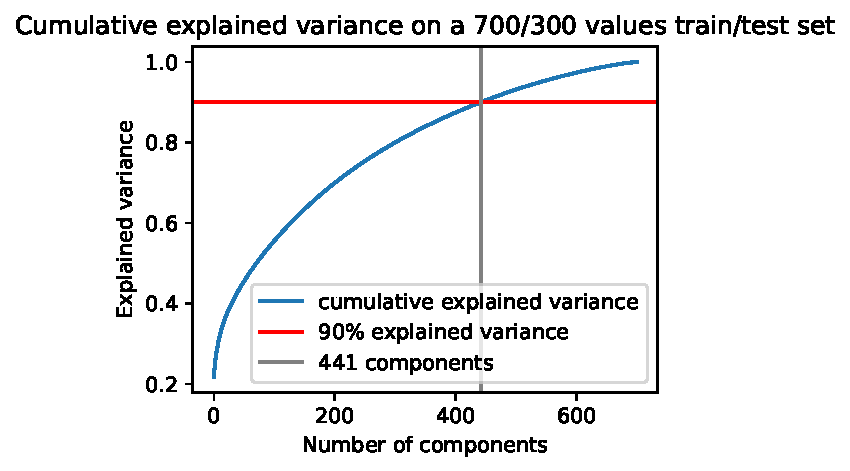
\includegraphics[width=7cm]{images/Eigendocs/Eval-Params/cumulative_explained_variance.pdf}}}%
    \qquad
    \subfloat[\centering The reconstruction error \ac{rmse} calculated for different values of $m$. Around 13 is a \textcolor{red}{"knee"}.]
    {{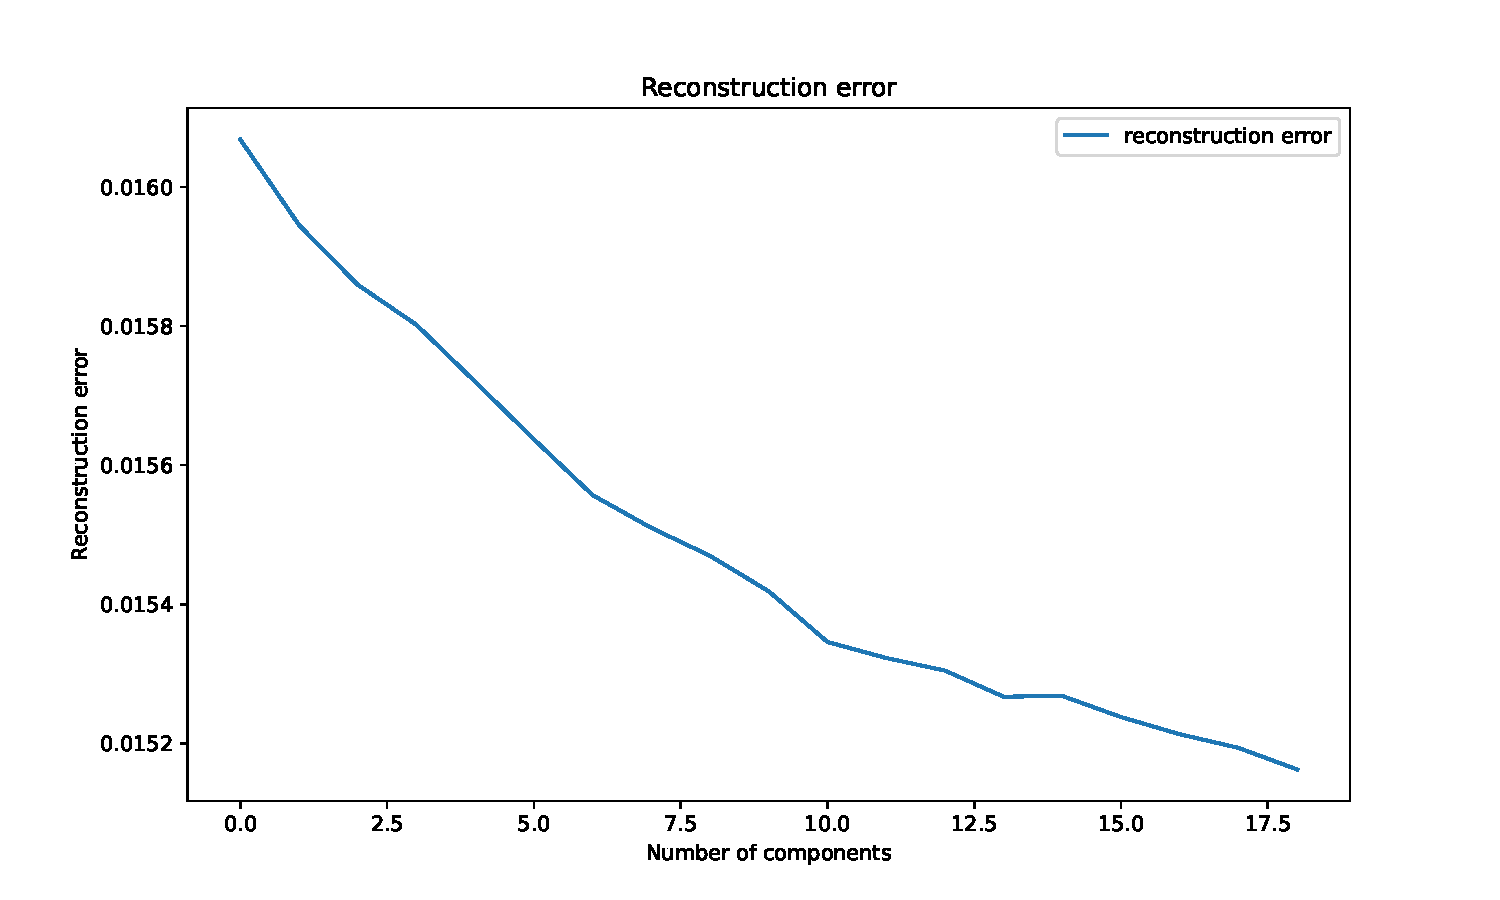
\includegraphics[width=7cm]{images/Eigendocs/Eval-Params/reconstruction error_eigendocs.pdf} }}%
    \caption{Two approaches in the literature to determine the number of \eigenfaces{} $m$ used to compress the input images.}%
    \label{fig:det_n_comp}%
\end{figure}

% calculation of eigenvectors of covariance matrix C
In order to reduce calculation complexity, $C$ is approximated.
% 1997
\citeauthor{eigenfaces1997} propose the approximation $\textbf{C} \simeq \frac{1}{N}\sum_{k=1}^{N}\textbf{x}_{k}\textbf{x}_{k}^{T} = \frac{1}{N}\textbf{X}\textbf{X}^{T}$, 
with $\textbf{X} = \left[ \textbf{x}_{1}, \textbf{x}_{2}, ..., \textbf{x}_{N} \right]$, $\textbf{x}_i \in \mathbb{R}^{n}$ \cite{eigenfaces1997}.

Finding the eigenvectors of $\textbf{X}\textbf{X}^{T}$ is still computationally expensive, since $\textbf{X}\textbf{X}^{T}$ is a $n$ by $n$ matrix.
According to \citeauthor{eigenfaces1997}, the eigenvectors of $\textbf{X}\textbf{X}^{T}$ can be calculated by using the eigenvectors of $\textbf{X}^{T}\textbf{X}$.
The eigenvalues $\textbf{e}_i \in \mathbb{R}^{n}$ of $\textbf{X}\textbf{X}^{T}$ can be derived from the eigenvectors $\textbf{v}_i \in \mathbb{R}^{N}$ of $\textbf{X}^{T}\textbf{X}$ by 
$\textbf{e}_i = \frac{1}{\sqrt{\lambda_i}}\textbf{X}\textbf{v}_i$ as discussed in more detail in \cite{eigenfaces1997}.
Hence, the problem is reduced to a $N$ by $N$ matrix, which is computationally less expensive to solve, since $N \ll n$.
Eigenvectors can be calculated using \ac{svd} \cite{eigenfaces1997}.

% classification/ compare
In the literature, face images are classified by comparing their position in the face space with those of already known faces \cite{eigenfaces1991}.
% performance 
According to \cite{eigenfaces1991}, this approach performs well on datasets with little variation in pose, lighting and facial expression.
However, \Citeauthor{eigenfaces1997} state, that the performance deteriorates if the variations increase since the changes introduce a bias 
that makes the distance function used to make classifications a no longer reliable measure.



\section{Clustering}\label{sec:clustering}

Clustering is used in a variety of domains to group data into meaningful subclasses, i.e. clusters \cite{OPTICS2013, OPTICS2014, OPTICS_kMeans_2016}.
According to \citeauthor{OPTICS2013}, common domains include anomaly detection, noise filtering, document clustering and image segmentation. 
The objective is to find clusters, which have a low inter-class similarity and a high intra-class similarity \cite{OPTICS2013}.
The similarity is measured by a distance function, which is dependent on the data type. 
Common distance functions are the Euclidean distance, the Manhattan distance and the Minkowski distance \cite{OPTICS_kMeans_2016}.

There are multiple clustering techniques, which can be divided into four categories \cite{OPTICS2016}: 
\begin{itemize}
    \item \textbf{Hierarchical clustering}:
    Algorithms, that create spherical or convex-shaped clusters, possibly naturally occurring. 
    A terminal condition has to be defined beforehand.
    Examples include CLINK, SLINK \cite{OPTICS2014} and \ac{optics} \cite{OPTICS2013}.

    \item \textbf{Partitional based clustering}: 
    Algorithms, that partition the data into $k$ clusters, whereas $k$ is given apriori.
    Clusters are shaped in a spherical manner, are similar in size and not necessarily naturally occurring.
    KMeans is a popular example of a partitional-based clustering algorithm.

    \item \textbf{Density based clustering}:
    Density is defined as the number of objects within a certain distance of each other \cite{OPTICS_kMeans_2016}.
    The resulting clusters can be of arbitrary shape and size.
    The algorithm usually chooses the optimal number of clusters given the input data.
    However, some algorithms are sensitive to input parameters, such as radius, minimum number of points and threshold.
    Popular examples are \ac{dbscan} and \ac{optics}.
    
    \item \textbf{Grid based clustering}:
    Similar to density-based clustering, but according to \citeauthor{OPTICS2016} better than density-based clustering.
    Examples include flexible grid-based clustering \cite{OPTICS2014}.
    
\end{itemize}

Multiple approaches listed below use the term \textit{$\varepsilon$-neighbourhood}, which is defined as the set of all objects within a certain distance $\varepsilon$ of a given object \cite{OPTICS2013}.
In other words: $N_\varepsilon (x) = \left\{ y \in X | dist(x,y) \le \varepsilon, y \neq x \right\}$, $\varepsilon$ being the so-called generating distance.


\subsection{KMeans}\label{subsec:kmeans}

KMeans partitions the data into $k \in \mathbb{N}$  clusters, $k$ is given apriori \cite{OPTICS_kMeans_2016}. %
First, $k$ centroids, i.e. cluster centres, are randomly initialized.
Then, the objects are assigned to the closest centroid.
Afterwards, the centroids are updated by calculating the mean of the assigned objects.
The process is repeated until the terminating condition, for instance, no more change in the clusters, is met \cite{OPTICS_kMeans_2016}.
By iteratively reassinging the objects to the closest centroid and updating the centroids, 
the algorithm minimizes the within-cluster sum of squared errors $E$, i.e. the sum of squared distances between objects in a cluster and their centroid $\mu_{i}$, 
calculated in \autoref{eq:kmeans-error} from \cite{OPTICS_kMeans_2016}, 
where $C_{i}$ is the $i$-th cluster.

\begin{equation}
    E = \sum_{i=1}^{k} \sum_{x \in C_{i}}\left\|x-\mu_{i}\right\|^{2}
\label{eq:kmeans-error}
\end{equation}

\citeauthor{OPTICS_kMeans_2016} claim, that KMeans does not identify outliers.


\subsection{DBSCAN}\label{subsec:dbscan}

The clusters identified by \ac{dbscan} have a high density and are separated by low-density regions \cite{OPTICS_kMeans_2016}.
In order to create clusters of minimum size and density, \ac{dbscan} distinguishes between three types of objects \cite{OPTICS_kMeans_2016}:

\begin{itemize}
    \item \textbf{Core objects}: 
    An object $x$ with at least $minPts \in \mathbb{N}$ objects in its $\varepsilon$-neighbourhood $N_\varepsilon(x)$, i.e. $| N_\varepsilon (x) | \geq minPts$ is true \cite{OPTICS2013}.

    \item \textbf{Border objects}: 
    An object with less than $minPts$ objects in its $\varepsilon$-neighbourhood, which is in the $\varepsilon$-neighbourhood of a core object.

    \item \textbf{Noise objects}: 
    An object, which is neither a core object nor a border object.
\end{itemize}

\citeauthor{OPTICS_kMeans_2016} define $y \in X$ as \textit{directly density reachable} from $x \in X$, if $y$ is in the $\varepsilon$-neighbourhood of core object $x$ \cite{OPTICS_kMeans_2016}.
Moreover, a point $y \in X$ is \textit{density reachable} from $x \in X$, if there is a chain of objects $x_1, ..., x_n$ with $x_1 = x$ and $x_n = y$, 
which are directly density reachable from each other as displayed in \autoref{fig:density_reachable} \cite{OPTICS_kMeans_2016}.

\begin{figure}[htp] % htp = hier (h), top (t), oder auf einer eigenen Seite (p).
    \centering
    \includesvg[width=0.2\textwidth]{images/density_reachable}
    \caption{Density reachability cf. \cite{OPTICS1999}.
    The point $y \in X$ is density reachable from $x \in X$, since there is a chain of directly density reachable objects $x, o, y$.
    }
    \label{fig:density_reachable}
\end{figure}

The points $x \in X$ and $y \in X$ are said to be \textit{density connected}, if there is an object $o$, from which both $x$ and $y$ are density reachable \cite{OPTICS_kMeans_2016}.
Density connectivity is visualized in \autoref{fig:density_connected}.

\begin{figure}[htp] % htp = hier (h), top (t), oder auf einer eigenen Seite (p).
    \centering
    \includesvg[width=0.2\textwidth]{images/density_connected}
    \caption{Density connectivity cf. \cite{OPTICS1999}.
    The objects $x$ and $y$ are density connected since there is an object $o$, from which both $x$ and $y$ are density reachable.
    }
    \label{fig:density_connected}
\end{figure}

The \ac{dbscan} algorithm starts by labelling all objects as core, border or noise points.
Then, it eliminates noise points and links all core points, which are within each other's neighbourhood \cite{OPTICS_kMeans_2016}.
Groups of connected core points form a cluster \cite{OPTICS_kMeans_2016}.
In the end, every border point is assigned to a cluster \cite{OPTICS_kMeans_2016}.
The non-core point cluster assigning is non-deterministic \cite{OPTICS2013}.
This algorithm creates clusters as a maximal set of density-connected points \cite{OPTICS_kMeans_2016}.

According to \citeauthor{OPTICS_kMeans_2016}, \ac{dbscan} can identify outliers or noise.
However, the algorithm is sensitive to the input parameters $minPts$ and $\varepsilon$ and has difficulties distinguishing closely located clusters \cite{OPTICS_kMeans_2016}.
Moreover, if one wants to obtain hierarchical clustering, one has to run the algorithm multiple times with different $\varepsilon$, which is expensive in terms of memory usage \cite{OPTICS2013}.



\subsection{\acs*{optics}}\label{subsec:optics}

\ac{optics} does not return an explicit clustering, but rather a density-based clustering structure of the data, 
which is equivalent to clustering results of a broad range of parameters \cite{OPTICS1999}.
\citeauthor{OPTICS1999} claim that real-world datasets cannot be described by a single global density, since they often consist of different local densities, 
as displayed in \autoref{fig:diff_density_cluster}.

\begin{figure}[htp] % htp = hier (h), top (t), oder auf einer eigenen Seite (p).
    \centering
    \includesvg[width=0.4\textwidth]{images/diff_density_cluster}
    \caption{Clusters of different densities cf. \cite{OPTICS1999}.
    Since $C_1$ and $C_2$ have different densities than $A$ and $B$, a clustering algorithm using one global density parameter would detect the clusters $A$, $B$ and $C$, 
    rather than $A$, $B$, $C_1$ and $C_2$ .
    }
    \label{fig:diff_density_cluster}
\end{figure}

Opposed to \ac{dbscan}, \ac{optics} is able to detect clusters of varying densities \cite{OPTICS2014}.
\ac{optics} produces an order of the elements according to the distance to the already added elements \cite{OPTICS2014, OPTICS2013}:
The first element added to the order list is arbitrary.
%$\varepsilon$ defines the neighbourhood radius, i.e. the maximum distance between two elements, which are still considered to be in the same neighbourhood \cite{OPTICS_kMeans_2016}.
The order list is iteratively expanded by adding the element of the $\varepsilon$-neighbourhood to the order list, which has the smallest distance to any of the elements already in the order list.
Hence, clusters with higher density, i.e. lower $\varepsilon$, are added first (prioritized) \cite{OPTICS_kMeans_2016, OPTICS1999}.
When there are no more elements in the $\varepsilon$-neighbourhood to add, the process is repeated for the other clusters.
The non-core point cluster assigning is non-deterministic \cite{OPTICS2013}.

\begin{equation}
    RD(y) = \left\{
    \begin{array}{ll}
    \textrm{NULL} & \, \textrm{if |}N_\varepsilon (x)| < minPts \\
    max(core\_dist(x), dist(x,y)) & \, \textrm{otherwise} \\
    \end{array}
    \right. 
    \label{eq:optics-reachability-distance}
\end{equation}

\ac{optics} saves the reachability distance $RD(y)$, as calculated in \autoref{eq:optics-reachability-distance} from \cite{OPTICS2013},
with core distance core\_dist being the minimal distance $\varepsilon^{min}$ such that $| N_{\varepsilon^{min}} (x) | \geq minPts$ 
(the distance to the $minPts^{th}$ point in $N_\varepsilon$) or NULL else, 
of each element to its predecessor in the order list and thus, 
a representation of the density necessary to keep two consecutive objects in the same cluster \cite{OPTICS2013}.
If $\varepsilon < RD(y)$, then $y$ is not density reachable from any of its predecessors and thus, 
one can determine whether two points are in the same cluster for given information saved by \ac{optics} \cite{OPTICS2013, OPTICS1999}.
If the core distance of an element is not NULL, i.e. it is a core object, and it is not density reachable from its predecessors, it is the start of a new cluster \cite{OPTICS1999}.
Otherwise, the element is a noise point \cite{OPTICS1999}.
According to \citeauthor{OPTICS2013}, the algorithm builds a spanning tree, which enables obtaining the clusters for a given $\varepsilon$ by returning the connected components 
of the spanning tree after omitting all edges with $\varepsilon < RD(y)$ \cite{OPTICS2013}.
The relationship between $\varepsilon$, cluster density and nested density-based clusters is displayed in \autoref{fig:nested_density_cluster}.

% nested clusters, eps, fixed minPts
\begin{figure}[htp] % htp = hier (h), top (t), oder auf einer eigenen Seite (p).
    \centering
    \includesvg[width=0.5\textwidth]{images/nested_density_cluster.svg}
    \caption{The relationship between $\varepsilon$, cluster density and nested density-based clusters cf. \cite{OPTICS1999}.
    For a constant $minPts$, clusters with higher density such as $C_1$, $C_2$ and $C_3$, i.e. a low $\varepsilon_2$ value, 
    are completely contained in lower density clusters such as $C$ given $\varepsilon_1 > \varepsilon_2$.
    This idea forms the basis of \ac{optics} of expanding clusters iteratively and thus, 
    enables the detection of clusters for a broad range of neighbourhood radii $0 \le \varepsilon_i \le \varepsilon$.
    }
    \label{fig:nested_density_cluster}
\end{figure}

Hence, this procedure enables the extraction of clusters for arbitrary $0 \le \varepsilon_i \le \varepsilon$ \cite{OPTICS_kMeans_2016, OPTICS1999}.
According to \citeauthor{OPTICS2013}'s work, even though the clustering algorithm is expensive the extraction only needs linear time.
According to \cite{OPTICS1999}, the algorithm yields good results if the input parameters $minPts$ and $\varepsilon$ are "large enough" and thus, the algorithm is rather insensitive to the input parameters.

% effect of eps (reachability plot)
The smaller $\varepsilon$ is chosen, the more objects will be identified as noise and thus, the algorithm will not identify clusters with low density, 
since some objects only become core objects for a larger $\varepsilon$ \cite{OPTICS1999}.
According to \citeauthor{OPTICS1999}, the optimal value for $\varepsilon$ creates one cluster for most of the objects with respect to a constant $minPts$,
since information about all density-based clusters for $\varepsilon_i < \varepsilon$ is preserved.
A heuristic for choosing $\varepsilon$ based on the expected $k$-nearest neighbour distance is presented in \cite{OPTICS1999}.

% effect of minPts (reachability plot)
High values for $minPts$ smoothen the reachability curve, even though the overall shape stays roughly the same \cite{OPTICS1999}.
According to \citeauthor{OPTICS1999}, the optimal value for $minPts$ is between 10 and 20.



\section{Database Elasticsearch}\label{subsec:db}

% introduction, users
\databaseName{} is a widely used non-relational database, which was designed to store and perform full-text search on a large corpus of unstructured data \cite{Elasticsearch2017}.
This open-source distributed document-driven database system is built in Java and is based on the Apache Lucene (Java) library for high-speed full-text search \cite{Elasticsearch2017, Elasticsearch2019}.
According to \citeauthor{Elasticsearch2019}, \databaseName{} provides Wikipedia's full-text search and suggestions as well as Github's code search and Stack Overflow's geolocation queries and related questions.
It enables near real-time search by index refreshing periods of one second.
Needless to say, \databaseName{} is qualified to handle Big Data.

% structure
\databaseName{}'s entries, i.e. documents, are stored in logical units, so-called indices.
% index
As stated by \citeauthor{Elasticsearch2019} and \citeauthor{Elasticsearch2017}, the indices are structured similarly to Apache Lucene's inverted index format.
An index can be spread into multiple nodes.
A node is single running instance of \databaseName{} \cite{Elasticsearch2019}.
An index is divided into one or more shards, which can be stored on different servers and enable parallelization \cite{Elasticsearch2019}.

% document
\databaseName{} indices' entries are documents, which are saved in a \ac{json} format \cite{Elasticsearch2017}.
A document's fields and field types are defined by the user when initializing the database index.
By default, every field of a document is indexed and searchable \cite{Elasticsearch2019}.

% Replicas
Replicas are copies of shards, which create redundancy and thus, ensure availability \cite{Elasticsearch2019}.

% query (endpoints)
% get: search id
By specifying the unique \texttt{\_id} of a document and the database \texttt{index}, it is possible to retrieve a specific document from the database using the \texttt{GET \ac{api}}.
The query is real-time by default.
The parameters \texttt{\_source\_excludes} or \texttt{\_source\_includes} may be used to exclude or include specific fields of the document in the response \cite{Elasticsearch-get}.

% full-text search
The keyword used when performing a full-text search is \texttt{match}.
To query for a specific value, one has to specify the \texttt{<field>} of interest and the query value.

\databaseName{} preprocesses the query value before starting the search \cite{Elasticsearch-text-analyser}.
The default preprocessing steps of the so-called default analyzer include tokenization and lowercasing \cite{Elasticsearch-text-analyser}. 
Omitting stop words is disabled by default, but it is possible to provide custom stop words or use the English stop word list \cite{Elasticsearch-text-analyser}.
It is possible to create custom tokenizers, which split the query value into tokens of a certain maximum length.

Another useful feature of \databaseName{} is the multi-term synonym expansion.
When the user queries a specific phrase \databaseName{} expands the query to include synonyms of the query terms \cite{Elasticsearch-synonyms}.
The maximum number of expansion terms is set to 50 by default but can be configured by the user \cite{Elasticsearch-match}.
By default, the multi-terms synonym expansion option is enabled \cite{Elasticsearch-match}.

\databaseName{} also provides the option to perform fuzzy matching instead of exact search.
By enabling the fuzzy matching option, a \databaseName{} query consisting of for instance, \textit{Bahama} returns documents that have the word \textit{Bahamas}.
By default, this option is not enabled but can be enabled and configured individually by the user \cite{Elasticsearch-match}.


% knn-search
Another search option of \databaseName{} is the \ac{knn} search.
The return value of a \ac{knn} search is the \texttt{k} nearest neighbors in terms of a certain distance function of a query vector \cite{Elasticsearch-kNN-HNSW}.
The query is a dense vector of the same dimension as the (dense) vectors stored in the database.
According to \cite{Elasticsearch-knn}, the \ac{knn} either returns the exact brute-force nearest neighbors or approximate nearest neighbors calculated by the \ac{hnsw} algorithm \cite{Elasticsearch-kNN-HNSW, Elasticsearch-knn}.
\ac{hnsw} is a graph-based algorithm \cite{Elasticsearch-kNN-HNSW}.
The term \texttt{navigable} refers to the graphs used, which are graphs with (poly-)logarithmic scaling of links traversed during greedy traversal concerning the network size \cite{Elasticsearch-kNN-HNSW}.
The idea of a \texttt{hiercharical} algorithm is to create a multilayer graph, grouping links according to their link length, as displayed in \autoref{fig:hnsw-layer}. 
The search starts on the uppermost layer, i.e. the layer containing the longest links, greedily traversing the layer until reaching the local minimum.
It uses this local minimum as the starting point at the next lower layer and the process is repeated until the lowest layer is reached \cite{Elasticsearch-kNN-HNSW}.
The layers of the graph are built incrementally, and a neighbour selection heuristic, as depicted in \autoref{fig:hnsw-heuristic}, not only creates links between close elements, 
but also between isolated clusters to ensure global connectivity \cite{Elasticsearch-kNN-HNSW}.

\begin{figure}[htp] % htp = hier (h), top (t), oder auf einer eigenen Seite (p).
    \centering
    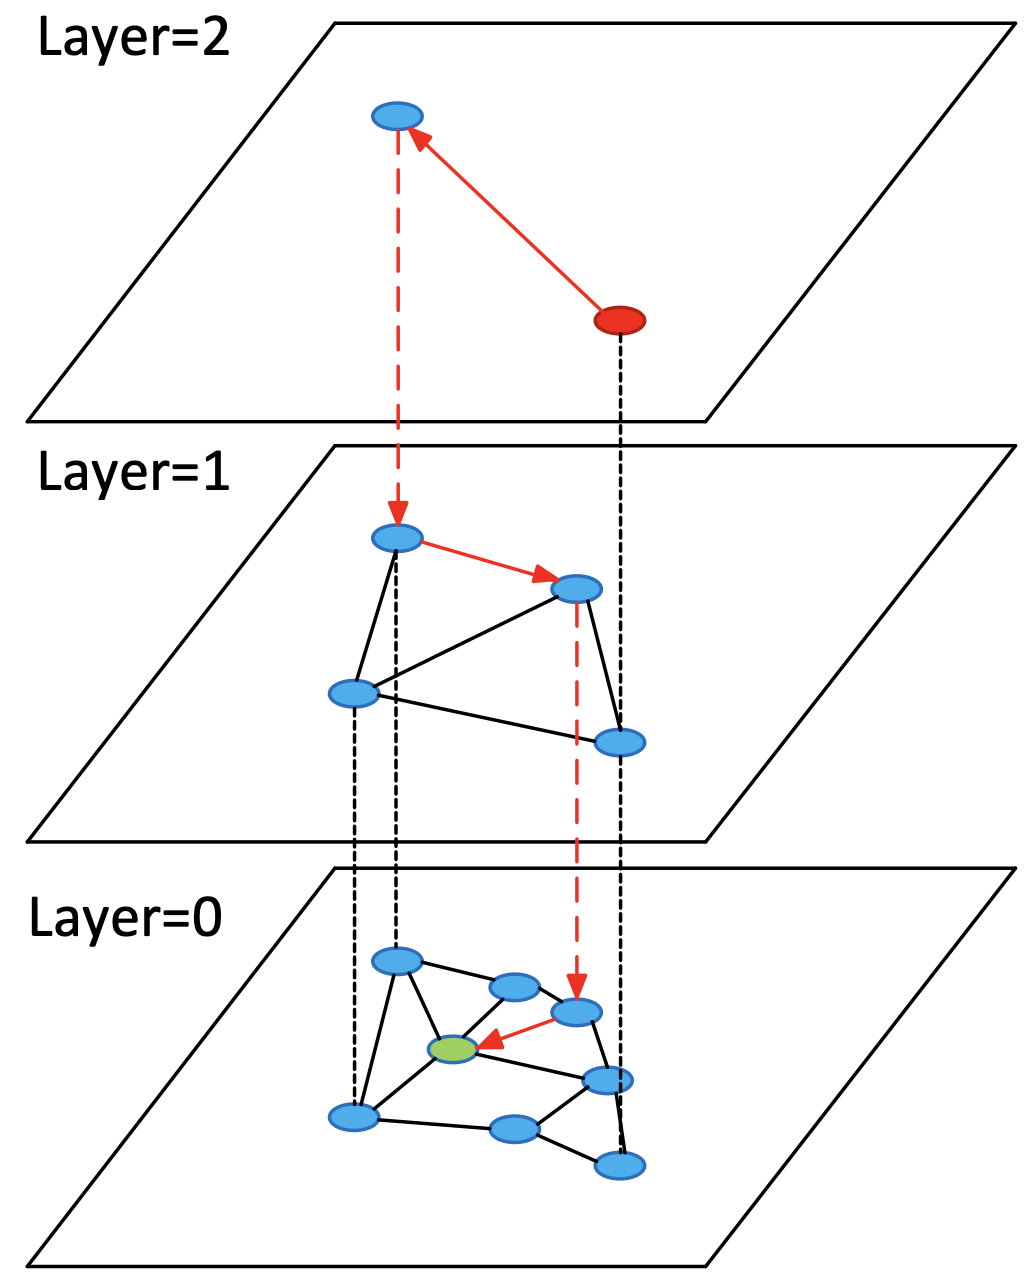
\includegraphics[width=0.3\textwidth]{images/HNSW-layer.png}
    \caption{Structure of \ac{hnsw} layer from \cite{Elasticsearch-kNN-HNSW}.
    The search starts on the uppermost layer, i.e. the layer containing the longest links, greedily traversing the layer until reaching the local minimum.
    The local minimum is used as the starting point at the next lower layer and the process is repeated until the lowest layer is reached.
    }
    \label{fig:hnsw-layer}
\end{figure}

\begin{figure}[htp] % htp = hier (h), top (t), oder auf einer eigenen Seite (p).
    \centering
    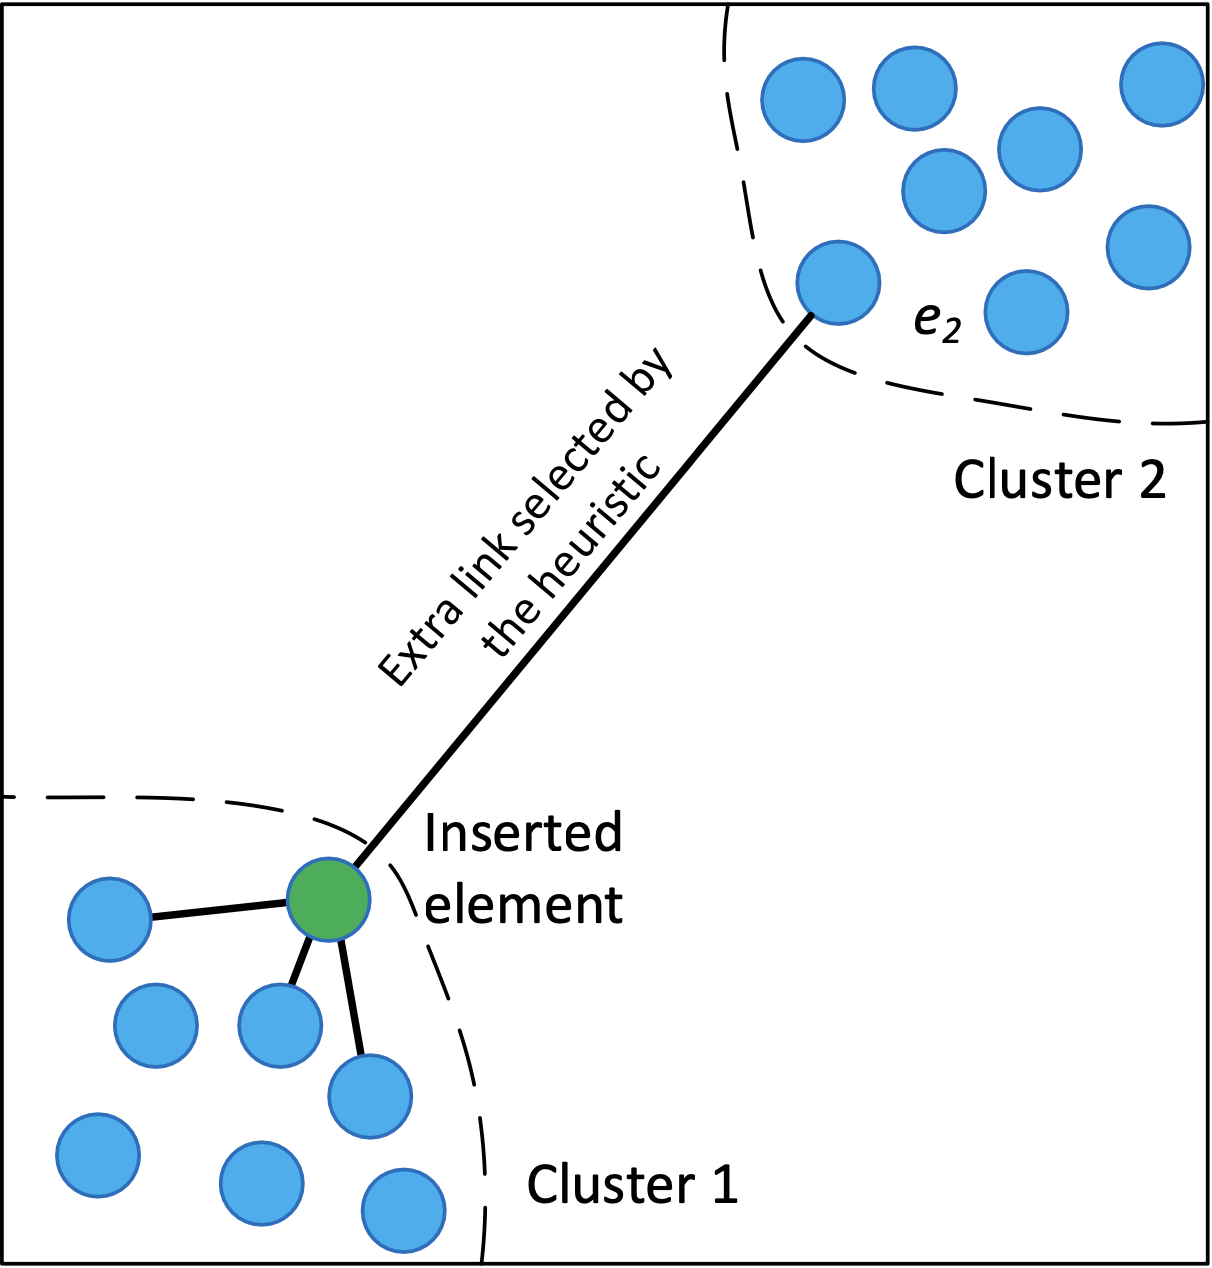
\includegraphics[width=0.3\textwidth]{images/HNSW-neighbour-selection-heuristic.png}
    \caption{Neighbour selection heuristic of \ac{hnsw} from \cite{Elasticsearch-kNN-HNSW}.
    The heuristic creates diverse links, i.e. links between close elements (e.g., green circle and elements in cluster 1) 
    and between isolated clusters (e.g., green circle and $e_2$) to ensure global connectivity.
    }
    \label{fig:hnsw-heuristic}
\end{figure}

In order to perform the \ac{knn} search on a \texttt{<field>} it has to be of type \texttt{dense\_vector}, indexed and a \texttt{similarity} measure has to be defined when initializing the database \cite{Elasticsearch-knn}.


\databaseName{}'s \ac{knn} implementation not only allows literal matching on search terms but also semantic search \cite{Elasticsearch-knn}.

Besides \databaseName{}, the elastic stack offers other tools, for instance, Kibana, which provides a user interface to manage different models.
After saving a model in Kibana, it is possible to create a text embedding ingest pipeline, which embeds new documents or reindexes existing documents \cite{Elasticsearch-knn-embedding}.




\section{\flask{}}\label{sec:BE_flask}

% introduction
\flask{} is open source and written in Python by Armin Ronancher in 2004 \cite{flask2015, mvc_flask2019}.
According to \citeauthor{flask_book2015} and \citeauthor{mvc_flask2019}, \flask{} is one of the most popular Python web frameworks.
It provides powerful libraries for core functionality such as routing, templating, and \ac{http} request parsing \cite{flask_book2015}.
It is extensible and thus, can be extended with additional plugins without affecting the internal structure of the existing system \cite{flask2015}.

% technical details
\flask{} uses the Jinja Template Engine for template files including \ac{html} pages,
whereas static files such as \ac{css} files are handeled using the Werkzeug WSGI toolkit \cite{flask2015}.
According to \citeauthor{flask2015}, Jinja is modeled after the Django template system.
Werkzeug implements, for instance, requests and response objects \cite{mvc_flask2019}.

% initialization
All requests received from clients are passed to an instance of the \flask{} application \cite{flask_book2018}.
Hence, the first step is to create an instance of the \flask{} class, such as done in \lst{lst:flask_app_init}.

\begin{listing}[htp]
    \begin{minted}{python3}
    app = Flask(__name__)
    \end{minted}
    \caption{Initialization of \flask{} application instance.
    }
    \label{lst:flask_app_init}
\end{listing}

% routing
Clients send requests to the web server, which passes them to the \flask{} application instance.
The queries are then routed to the corresponding functions.
Routing is the process of mapping \ac{url} paths to functions \cite{flask_book2018}.
To define a route, the \texttt{route} decorator is used as displayed in \lst{lst:flask_routing}.

\begin{listing}[htp]
    \begin{minted}{python3}
    @api.route('/documents/<id>', endpoint='document')
    class Document(Resource):
        def get(self, id):
            elastic_search_client = Elasticsearch(CLIENT_ADDR)
            return query_database.get_doc_meta_data(elastic_search_client, 
                doc_id=id)
    \end{minted}
    \caption{Exemplartary definition of a function to display routing with \flask{}.
    The \texttt{route} decorator is used to define the \ac{url} path.
    }
    \label{lst:flask_routing}
\end{listing}

\acs{url} can contain dynamic components, which are enclosed in \texttt{<>} angle brackets.
The values of these components are passed to the function as arguments \cite{flask_book2018}.
By default, dynamic components are of type \texttt{string}.
However, other types including \texttt{int} and \texttt{float} are supported \cite{flask_book2018}.

% dev server
During development, the \flask{} application can be run using \texttt{flask run} to start the built-in development web server \cite{flask_book2018}.
By enabling debug mode, the server automatically reloads the application when changes are detected \cite{flask_book2018}.

% endpoints
An endpoint is a class with certain methods, which can be accessed using \ac{http} requests.
Every endpoint can have a \texttt{GET}, \texttt{PUT} and a \texttt{DELETE} method \cite{flask2018}.
The \texttt{GET} method is used to retrieve data from the server, whereas the other methods are used to either insert or delete data.

    \chapter{Implementation}\label{ch:implementation}


\section{Slurm}\label{subsec:slurm}

Slurm is an open-source management tool for Linux clusters \cite{slurm-online}.
It allocates resources, i.e. compute nodes, and provides the means to start, execute and monitor jobs \cite{slurm-online, slurm2003}.

The so-called slurm daemons control nodes, partitions, jobs and job steps \cite{slurm-online}.
According to \citeauthor{slurm-online}, a partition is a group of nodes and a job is the allocation of resources, i.e. compute nodes, to a user for a limited period of time.
A basic visualization of the architecture is given in \autoref{fig:slurm-architecture}.

\begin{figure}[htp] % htp = hier (h), top (t), oder auf einer eigenen Seite (p).
    \centering
    \includesvg[width=0.7\textwidth]{images/slurm_architecture}
    \caption{Slurm architecture. The management node has a \texttt{slurmctld} daemon, while every compute node has a \texttt{slurmd} daemon.
    The nodes communicate.
    The user can use certain commands, for instance \texttt{srun} and \texttt{squeue}, anywhere on the cluster.
    }
    \label{fig:slurm-architecture}
\end{figure}


\section{Elasticsearch}\label{subsec:impl-db}
First, the content of the database is described, then, the initialization, insertion and updating process of filling the database are explained 
and finally, the querying is presented.

% content
\subsubsection*{Content of the database}
In this work, the database is filled once with data from a large unstructured corpus of \ac{pdf} files.
After the initialization of the database, it is used for queries. 
Therefore, the workflow is completely offline.

The index \textit{Bahamas} stores different embeddings of the text layer information and metadata of the documents.
As depicted in \autoref{fig:pdf2db}, not only textual information is stored in the database, 
but also information about the appearance of the first page of the \ac{pdf}.
The structure of the index is presented in \autoref{tbl:Elasticsearch-fields}.

\begin{table}[]
    \caption{Fields in \databaseName{} database in index \textit{Bahamas}.}
    \begin{tabular}{|
    >{\columncolor[HTML]{EFEFEF}}l |p{0.63\textwidth}|}
    \hline
    \cellcolor[HTML]{C0C0C0}\textbf{field name} & \cellcolor[HTML]{C0C0C0}\textbf{field description}                                     \\ \hline
    \_id                                        & Unique identifier of document \texttt{i}. The identifier is generated by the sha256 hash algorithm from hashlib.\\ \hline
    doc2vec                                     & 55 dimensional doc2vec embedding of \texttt{i}.                                                          \\ \hline
    sim\_docs\_tfidf                            & sim\_docs\_tfidf embedding + all-zero flag of \texttt{i}. The all-zero flag is one if the \ac{tfidf} embedding consists of only zeros, zero else.\\ \hline
    google\_univ\_sent\_encoding                & 512 dimensional google\_univ\_sent\_encoding embedding of \texttt{i}.                                     \\ \hline
    huggingface\_sent\_transformer              & 384 dimensional huggingface\_sent\_transformer embedding of \texttt{i}.                                  \\ \hline
    inferSent\_AE                               & inferSent\_AE embedding of \texttt{i}. Since the pretrained \infersent{} model embedding's dimension is 4096, the encoder of a trained \ac{ae} is added to reduce the dimension to 2048.                                                    \\ \hline
    pca\_image                                  & Two dimensional \ac{pca} version of first page image of \texttt{i}.                      \\ \hline
    pca\_optics\_cluster                        & Cluster of \texttt{i} identified by \acs{optics} on \ac{pca} version of image.            \\ \hline
    argmax\_pca\_cluster                        & Number of maximum \ac{pca} component as cluster of \texttt{i}.                            \\ \hline
    text                                        & Text of \texttt{i}.                                                                       \\ \hline
    path                                        & Path to \texttt{i}.                                                     \\ \hline
    \end{tabular}
    \label{tbl:Elasticsearch-fields}
\end{table}

\begin{figure}[htp] % htp = hier (h), top (t), oder auf einer eigenen Seite (p).
    \centering
    \includesvg[width=0.7\textwidth]{images/Elasticsearch/PDFs_to_database}
    \caption{\acp{pdf} to Database. 
    First, the data is preprocessed:
    The first page of a \ac{pdf} file is converted to an image and the complete text is extracted. 
    The images are stored in the database as well as the text and different embeddings of the text.
    }
    \label{fig:pdf2db}
\end{figure}

% initialize, insert, update
\subsubsection*{Initialization, insertion and updating}
To facilitate working with and running the code the initialization of the database is split into multiple steps.
As depicted in \autoref{fig:init_db}, first the database is initialized by defining the index name and the mappings, i.e. the field names, types and sizes.
This step is carried out using the keyword \texttt{create}.

\begin{figure}[htp] % htp = hier (h), top (t), oder auf einer eigenen Seite (p).
    \centering
    \includesvg[width=0.7\textwidth]{images/Elasticsearch/init_db.svg}
    \caption{Initialization and filling of the database.}
    \label{fig:init_db}
\end{figure}

Afterwards, the documents are created.
The initial creation of a document only defines the fields \texttt{id}, \texttt{text} and \texttt{path}.
In order to maximise efficiency when updating the database, the \databaseName{}'s built-in functionality \texttt{bulk} is used.
\texttt{bulk} sends chunks of multiple requests to the database.
As displayed in \lst{lst:db_bulk}, the \texttt{bulk} is called with the \databaseName{} client, 
a function which yields requests and parameters, which define the return values.
The structure of a function that yields requests is shown in \lst{lst:db_bulk_yield}.

\begin{listing}[htp]
    \begin{minted}{python3}
        bulk(client, create_document_aux(src_paths, client), stats_only= True)
    \end{minted}
    \caption{Usage of \databaseName{}'s helper functionality \texttt{bulk} to send multiple requests to the database in chunks.
    }
    \label{lst:db_bulk}
\end{listing}

\begin{listing}[htp]
    \begin{minted}{python3}
        def create_document_aux(src_paths: list, client: Elasticsearch):  
            for path in src_paths:           
                id = get_hash_file(path)
                if get_doc_meta_data(client, doc_id=id) is not None:
                    return
                text = pdf_to_str(path)
                yield { '_op_type': 'create',
                        '_index': 'bahamas',
                        '_id': id,
                        "text": text,
                        "path": path}
    \end{minted}
    \caption{Method that yields requests for \texttt{bulk}.
    The method checks if the document is already in the database and if not, it yields a request to create the document.
    }
    \label{lst:db_bulk_yield}
\end{listing}

The embeddings are added to the documents in a third step.
To make sure that it is possible to update embeddings individually without changing other fields, 
a method to insert the embeddings of a specific model for all documents is created.
The documents are updated using the \texttt{update} keyword and \texttt{bulk}.


% search
\subsubsection*{Queries}
The default analyzer is used for the full-text search since for instance configuring a maximum token length did not seem necessary or likely to improve the results.

\begin{listing}[htp]
    \begin{minted}{python3}
        results = elastic_search_client.search(
            index='bahamas', 
            size=count,
            from_=(page*count),
            query= {'match' : {
                        'text': {   'query':text,
                                    'fuzziness': 'AUTO',}
                    }, 
                }, source_includes=SRC_INCLUDES)
    \end{minted}
    \caption{Exemplartary query to an \databaseName database index.
    The number of results to return \texttt{size} and the start index of the results \texttt{from\_} is defined.
    To enable fuzzy search a value for \texttt{fuzziness} has to be defined. 
    }
    \label{lst:fuzzy_query}
\end{listing}

Moreover, the fuzzy matching option is set to \texttt{AUTO}, which means in terms of keyword or text fields that the allowed Levenshtein Edit Distance, 
i.e. number of characters changed to create an exact match between two terms, to be considered a match, is correlated to the length of the term \cite{Elasticsearch-fuzziness}.
By default, terms of length up to two characters must match exactly, terms of length three to five characters must have an edit distance of one and 
terms of length six or more characters must have an edit distance of two \cite{Elasticsearch-fuzziness}.
An exemplary query, which uses fuzzy search is given in \lst{lst:fuzzy_query}.

According to \citeauthor{Elasticsearch-kNN-HNSW}, one of \ac{knn} search's use cases is semantic document retrieval, which makes it a good fit for this task.
In this work, the approximate nearest neighbours search is used, since it is faster and the results are good enough for the use case of this work.
The similarity measure used in this work is the cosine similarity, which calculates the \texttt{\_score} of a document according to \autoref{eq:cosine-similarity-db} from \cite{Elasticsearch-kNN-similarity}, 
where \texttt{query} is the query vector and \texttt{vector} is the vector representation of the document in the database.
The other similarity measures provided by \databaseName{} are \texttt{l2\_norm} or 
so-called Euclidian distance and \texttt{dot\_product} which is the non-auto-normalized version of the \texttt{cosine} option.
Since cosine is not defined on vectors with zero magnitude, embeddings that can return all zero vector representations, such as sim\_docs\_tfidf, 
are enhanced with an all-zero flag before inserting them into the database.

\begin{equation}
    \frac{1 + \text{cosine}(\text{query}, \text{vector})}{2}
    \label{eq:cosine-similarity-db}
\end{equation}

In this work, the only tool from the elastic stack used is \databaseName{}.
Without Kibana, the used models are saved on disk as \ac{pkl} files.
Consequently, instead of using the \ac{knn} query structure for semantic search on embeddings provided by \databaseName{}, the normal \ac{knn} search on a field that contains an embedding is used.

\section{\eigendocs{}}\label{subsec:eigendocs}

% this work
\begin{figure}[htp] % htp = hier (h), top (t), oder auf einer eigenen Seite (p).
    \centering
    \includesvg[width=1.0\textwidth]{images/eigendocs}
    \caption{From \acp{pdf} to \eigendocs{}.
    Firstly, the first page of a document is converted to an image.
    Then the image is preprocessed:
    It is placed on a white canvas, to ensure all images have the same dimensions.
    Moreover, it is converted to greyscale.
    Afterwards, the 2d image is reshaped to a 1d array.
    Lastly, the image is compressed using \eigenfaces{}.
    }
    \label{fig:eigendocs_procedure}
\end{figure}

In this work, the \eigenfaces{} approach from \autoref{subsec:eigenface} is used to compress the images of the first page of documents.
The idea is that documents not only hold textual information but also visual information, such as layout, company logo or signature.
By mapping those images on a subspace, they ought to be grouped by visual similarity.
The procedure of the eigenface adaption \textit{eigendocs} is displayed in \autoref{fig:eigendocs_procedure}.

% procedure
The documents are first read from a directory. 
Subsequently, their first page is converted to an image and saved.
When initially filling the database, these images are read from their directory.
Firstly, the maximum height and width of all images in the corpus is calculated.
These dimension are used to create a white canvas for each image which forms the background.
Every image is placed in the upper left corner.
Hence, scaling is not necessary and thus, the portion of white pixels on the right and bottom side encodes the dimension of the former image.
Therefore, the relative size of images in the corpus is incooperated in the resulting representation fo the input images.

\begin{listing}[htp]
    \begin{minted}{python3}
        C = np.ones((max_w,max_h))
        C[:doc.shape[0],:doc.shape[1]] = rgb2gray(doc)
        documents.append(C.ravel())
    \end{minted}
    \caption{Preprocessing of the input images from \thesissupervisor{}.
    The background is a white canvas.
    The images are converted to one-dimensional greyscale values.}
    \label{lst:preproc_images}
\end{listing}

Afterwards, they are converted to greyscale images using \autoref{lst:rgb2grey}.
Before returning the image, the two-dimensional image vectors are converted to one-dimensional ones as displayed in the last line of \autoref{lst:preproc_images}.
The decomposition is transformed using \ac{pca} as displayed in \autoref{lst:pca_svd}.

\begin{listing}[htp]
    \begin{minted}{python3}
        0.299*img[:,:,0] + 0.587*img[:,:,1] + 0.114*img[:,:,2]
    \end{minted}
    \caption{Conversion of RGB pixel values to greyscale by a script from \thesissupervisor{}.}
    \label{lst:rgb2grey}
\end{listing}

\begin{listing}[htp]
    \begin{minted}{python3}
        pca = decomposition.PCA(n_components=n_components, whiten=True, 
            svd_solver="randomized")
    \end{minted}
    \caption{Initialization of the \ac{pca} instace used to compress the image data.
    In order to work according to the \eigenfaces{} approach a svd\_solver has to be used.
    }
    \label{lst:pca_svd}
\end{listing}




\section{\acl{ae}}\label{subsec:impl-autoencoder}

In this work, the \ac{ae} is used to reduce the dimensionality of the \infersent{} embedding.
Since the \infersent{} model is pretrained, it is not possible to change the dimensionality of the embedding without a considerably big effort,
i.e. retraining the model on a sufficiently large data corpus and reconfiguring the model's parameters.
Moreover, retraining the model would destroy the purpose of its presence in this work, which is to provide a pretrained model and thus, 
reducing the complexity of training an own model.
Therefore, it is not feasible to change the dimensionality of the \infersent{} embedding, but rather adding a supplementary layer after the model 
produce the final embedding.
Hence, the idea is to use the encoder of an \ac{ae} to reduce the dimensionality of the \infersent{} embedding.

The architecture and implementation from \lst{lst:impl_ae} was provided from 
\href{https://blog.paperspace.com/autoencoder-image-compression-keras/}{a blog post using keras}.
\autoref{fig:impl-encoder} \autoref{fig:impl-ae}

\begin{figure}[h] % htp = hier (h), top (t), oder auf einer eigenen Seite (p).
    \centering
    \includesvg[width=0.6\textwidth]{images/compression/autoencoder/encoder-impl.svg}
    \caption{Architecture of the encoder of the \ac{ae}}
    \label{fig:impl-encoder}
\end{figure}

\begin{figure}[h] % htp = hier (h), top (t), oder auf einer eigenen Seite (p).
    \centering
    \includesvg[width=1.0\textwidth]{images/compression/autoencoder/autoencoder-impl.svg}
    \caption{Architecture of the \ac{ae}}
    \label{fig:impl-ae}
\end{figure}

\begin{listing}[htp]
    \begin{minted}{python3}
    # Encoder
    x = layers.Input(shape=(input_shape), name="encoder_input")
    encoder_dense_layer1 = layers.Dense(units=300, name="encoder_dense_1")(x)
    encoder_activ_layer1 = layers.LeakyReLU(name="encoder_leakyrelu_1")(encoder_dense_layer1)
    encoder_dense_layer2 = layers.Dense(units=latent_dim, name="encoder_dense_2")(encoder_activ_layer1)
    encoder_output = layers.LeakyReLU(name="encoder_output")(encoder_dense_layer2)
    encoder = models.Model(x, encoder_output, name="encoder_model")

    # Decoder
    decoder_input = layers.Input(shape=(latent_dim), name="decoder_input")
    decoder_dense_layer1 = layers.Dense(units=300, name="decoder_dense_1")(decoder_input)
    decoder_activ_layer1 = layers.LeakyReLU(name="decoder_leakyrelu_1")(decoder_dense_layer1)
    decoder_dense_layer2 = layers.Dense(units=input_shape, name="decoder_dense_2")(decoder_activ_layer1)
    decoder_output = layers.LeakyReLU(name="decoder_output")(decoder_dense_layer2)
    decoder = models.Model(decoder_input, decoder_output, name="decoder_model")

    # Autoencoder
    ae_input = layers.Input(shape=(input_shape), name="AE_input")
    ae_encoder_output = encoder(ae_input)
    ae_decoder_output = decoder(ae_encoder_output)
    ae = models.Model(ae_input, ae_decoder_output, name="AE")
    ae.compile(loss="mse", optimizer=optimizers.legacy.Adam(learning_rate=0.0005))
    ae.fit(x_train, x_train, epochs=20, batch_size=256, shuffle=True, validation_data=(x_test, x_test))
    \end{minted}
    \caption{Architecture of \ac{ae} using \texttt{tensorflow.keras}. 
    }
    \label{lst:impl_ae}
\end{listing}

\section{\ac{tfidf}}\label{sec:impl-tfidf}

% overall architecture
The \ac{tfidf} model has to be initialized and trained on the data corpus to build the data-specific vocabulary.
An exemplary implementation is given in \lst{lst:impl-tfidf}.
The \texttt{TfidfVectorizer} is provided by the \texttt{scikit-learn} package.
When initializing the model, the parameters define not only the input type but also the way the data is preprocessed.
The \texttt{input} parameter defines the input type, i.e., \texttt{content} means that the input is a list of strings or bytes, 
whereas \texttt{file} assumes the input has a \texttt{read} method and \texttt{filename} denotes a list of filenames as input \cite{tfidf-vec-scikit-learn}.

The \texttt{preprocessor} parameter defines the preprocessing (string transformation) stage.
It is possible to override the default with a custom preprocessing function.
The parameters \texttt{min\_df} and \texttt{max\_df} define the minimum and maximum document frequency of a word in the corpus.
The default values are $1$, i.e. a term has to appear at least once, and $1.0$, i.e. a term appears at most in all documents, respectively \cite{tfidf-vec-scikit-learn}.

The implementation of \ac{tfidf} in \texttt{scikit-learn} is different from the original \ac{tfidf} definition.
By default, the \texttt{scikit-learn} implementation uses the \texttt{norm='l2'} parameter, i.e. the Euclidean norm \cite{tfidf-scikit-learn}.
The difference is the calculation of the \ac{idf} part, which is given in \autoref{eq:tfidf-scikit-learn} from \cite{tfidf-scikit-learn}.
The one is added to $M_{ij}$ due to the parameter \texttt{smooth\_id=True} by default to prevent zero divisions \cite{tfidf-scikit-learn}
and to avoid logarithmic divergences due to a zero argument \cite{glove2014}.
After calculating the \ac{tfidf} values, they are normalized by the Euclidean norm 
$v_{norm} = \frac{v}{\left\| v \right\|_{2}} = \frac{v}{\sqrt{v_1^{2} + v_2^{2} + ... + v_M^{2}}}$.

\begin{equation}
    \text{idf}(w_{ij}) = \log \frac{1 + M}{1 + M_{ij}} + 1    
    \label{eq:tfidf-scikit-learn}
\end{equation}

\begin{listing}[htp]
    \begin{minted}{python3}
        tfidf = TfidfVectorizer(input='content', 
                    preprocessor=TfidfTextPreprocessor().transform, min_df=3, 
                    max_df=int(len(docs)*0.07))
        tfidf.fit(documents)
    \end{minted}
    \caption{Initialization of the \ac{tfidf} model.
    Firstly, an instance of the \texttt{TfidfVectorizer} class is created.
    Secondly, the \texttt{fit} method is called to fit the model to the documents.
    }
    \label{lst:impl-tfidf}
\end{listing}

% pipeline
In this work, the text of the \acp{pdf} is first extracted, then preprocessed using a custom preprocessor and afterwards embedded using the \texttt{TfidfVectorizer},
which returns the \ac{tfidf} weights as embedding.
Before storing the \ac{tfidf} weights in the database, they are enhanced with an all-zero flag.
The all-zero flag ensures that no all-zero vectors are stored in the database by enhancing those that have a zero magnitude with a "1" entry and "0" otherwise.
All-zero \ac{tfidf} weights indicate that a document does not have any terms with the vocabulary in common.
Since the vocabulary is kept relatively small with respect to the number of different words in the data corpus to reduce the dimensionality of the embeddings, 
it is not unlikely that a document does not contain any of the vocabulary terms.
The all-zero flag is necessary because the cosine similarity used to query for similar documents in the database cannot handle vectors of zero magnitude.
The pipeline in \autoref{fig:tfidf_embedding} visualizes the steps.

\begin{figure}[h] % htp = hier (h), top (t), oder auf einer eigenen Seite (p).
    \centering
    \includesvg[width=1.0\textwidth]{images/TFIDF_embedding}
    \caption{\ac{tfidf} pipeline.
    Firstly, the text extracted from the documents is preprocessed using a custom preprocessor.
    Then the \ac{tfidf} are obtained from the \texttt{TfidfVectorizer}.
    Lastly, the all-zero flag is added to the \ac{tfidf} weights and they are stored in the database.
    }
    \label{fig:tfidf_embedding}
\end{figure}

% custom preprocessing
In this work, a custom preprocessing function is used.
The preprocessing steps are visualized in \autoref{fig:preprocessing} on an exemplary text.
Firstly, the accents are stripped from the text.
Then, all new line symbols are replaced with a whitespace.
Afterwards, the text is converted to lowercase.
Then the numbers are discretized, i.e. all numbers between 0 and 99999 are replaced with the string \texttt{SMALLNUMBER}, 
numbers bigger than 99999 are replaced with the string \texttt{BIGNUMBER} and floats are replaced with the string \texttt{FLOAT}.
The next step is to remove all punctuation symbols.
After that, the symbols for numbers are enclosed with pointed brackets, e.g. \texttt{<SMALLNUMBER>}.
Then, the text is tokenized, i.e. splitting at whitespaces, and stop words are omitted.
The stop word corpus used is provided by the \texttt{nltk} package and consists of common English stop words.
Afterwards, the tokens are lemmatized.
The lemmatizer used is \texttt{WordNetLemmatizer} from the \texttt{nltk} package.
In the end, the tokens are joined to a string again.


\begin{figure}[htp] % htp = hier (h), top (t), oder auf einer eigenen Seite (p).
    \centering
    \includesvg[width=1.1\textwidth]{images/TFIDF_preprocessing}
    \caption{\ac{tfidf} Preprocessing visualized using a example text. \textcolor{red}{TODO: nicht aktuell bzgl. small number - etc.}}
    \label{fig:preprocessing}
\end{figure}

\section{\ac{doc2vec}}\label{sec:impl-doc2vec}

\textcolor{red}{TODO: find out activation function, vector size, window size and training epoch and corpus of model used}

\section{\infersent{}}\label{sec:impl-infersent}

The \infersent{} model is based on PyTorch \cite{HfsentTrans2019}.

\textcolor{red}{W2V path}
% GloVe
The \infersent{} model is based on GloVe word embeddings.
GloVe introduces bias in terms of ageism, racism and sexism into the model \cite{UniversalSentEnc2018}.

\section{\ac{use}}\label{sec:impl-use}

The \ac{use} model is based on TensorFlow \cite{HfsentTrans2019}.

\section{\ac{sbert}}\label{sec:impl-sbert}

The \ac{sbert} model is based on PyTorch \cite{HfsentTrans2019}.

\subsection{Clustering using \ac{optics}}\label{subsec:impl-optics}

\begin{figure}[htp] % htp = hier (h), top (t), oder auf einer eigenen Seite (p).
    \centering
    \includesvg[width=0.5\textwidth]{images/OPTICS/OPTICS_procedure.svg}
    \caption{First, the first page of each document is converted to an image.
    Then the image is preprocessed, i.e. conversion to greyscale and resizing.
    }
    \label{fig:OPTICS_procedure}
\end{figure}

Similar to the approach from \cite{OPTICS1999}, \ac{optics} was used to cluster the images of the first page of documents in this work.
The procedure is displayed in \autoref{fig:OPTICS_procedure}.
There were two different preprocessing approaches:
\begin{enumerate}
    \item \label{pt:32}The images were first preprocessed to 32x32 greyscale pixels (cf. \cite{OPTICS1999}) as visualized in \autoref{fig:preprocessed_docs_32x32}
    and afterwards compressed to 13-dimensional vectors using \ac{pca}.
    \item \label{pt:eigendocs}The technique \eigendocs{} from \autoref{subsec:eigenface} 
    was used to compress the images to 13-dimensional greyscale images as displayed in \autoref{fig:preprocessed_docs_eigendocs}.
\end{enumerate}


% preprocessed images
\begin{figure}[htp] % htp = hier (h), top (t), oder auf einer eigenen Seite (p).
    \centering
    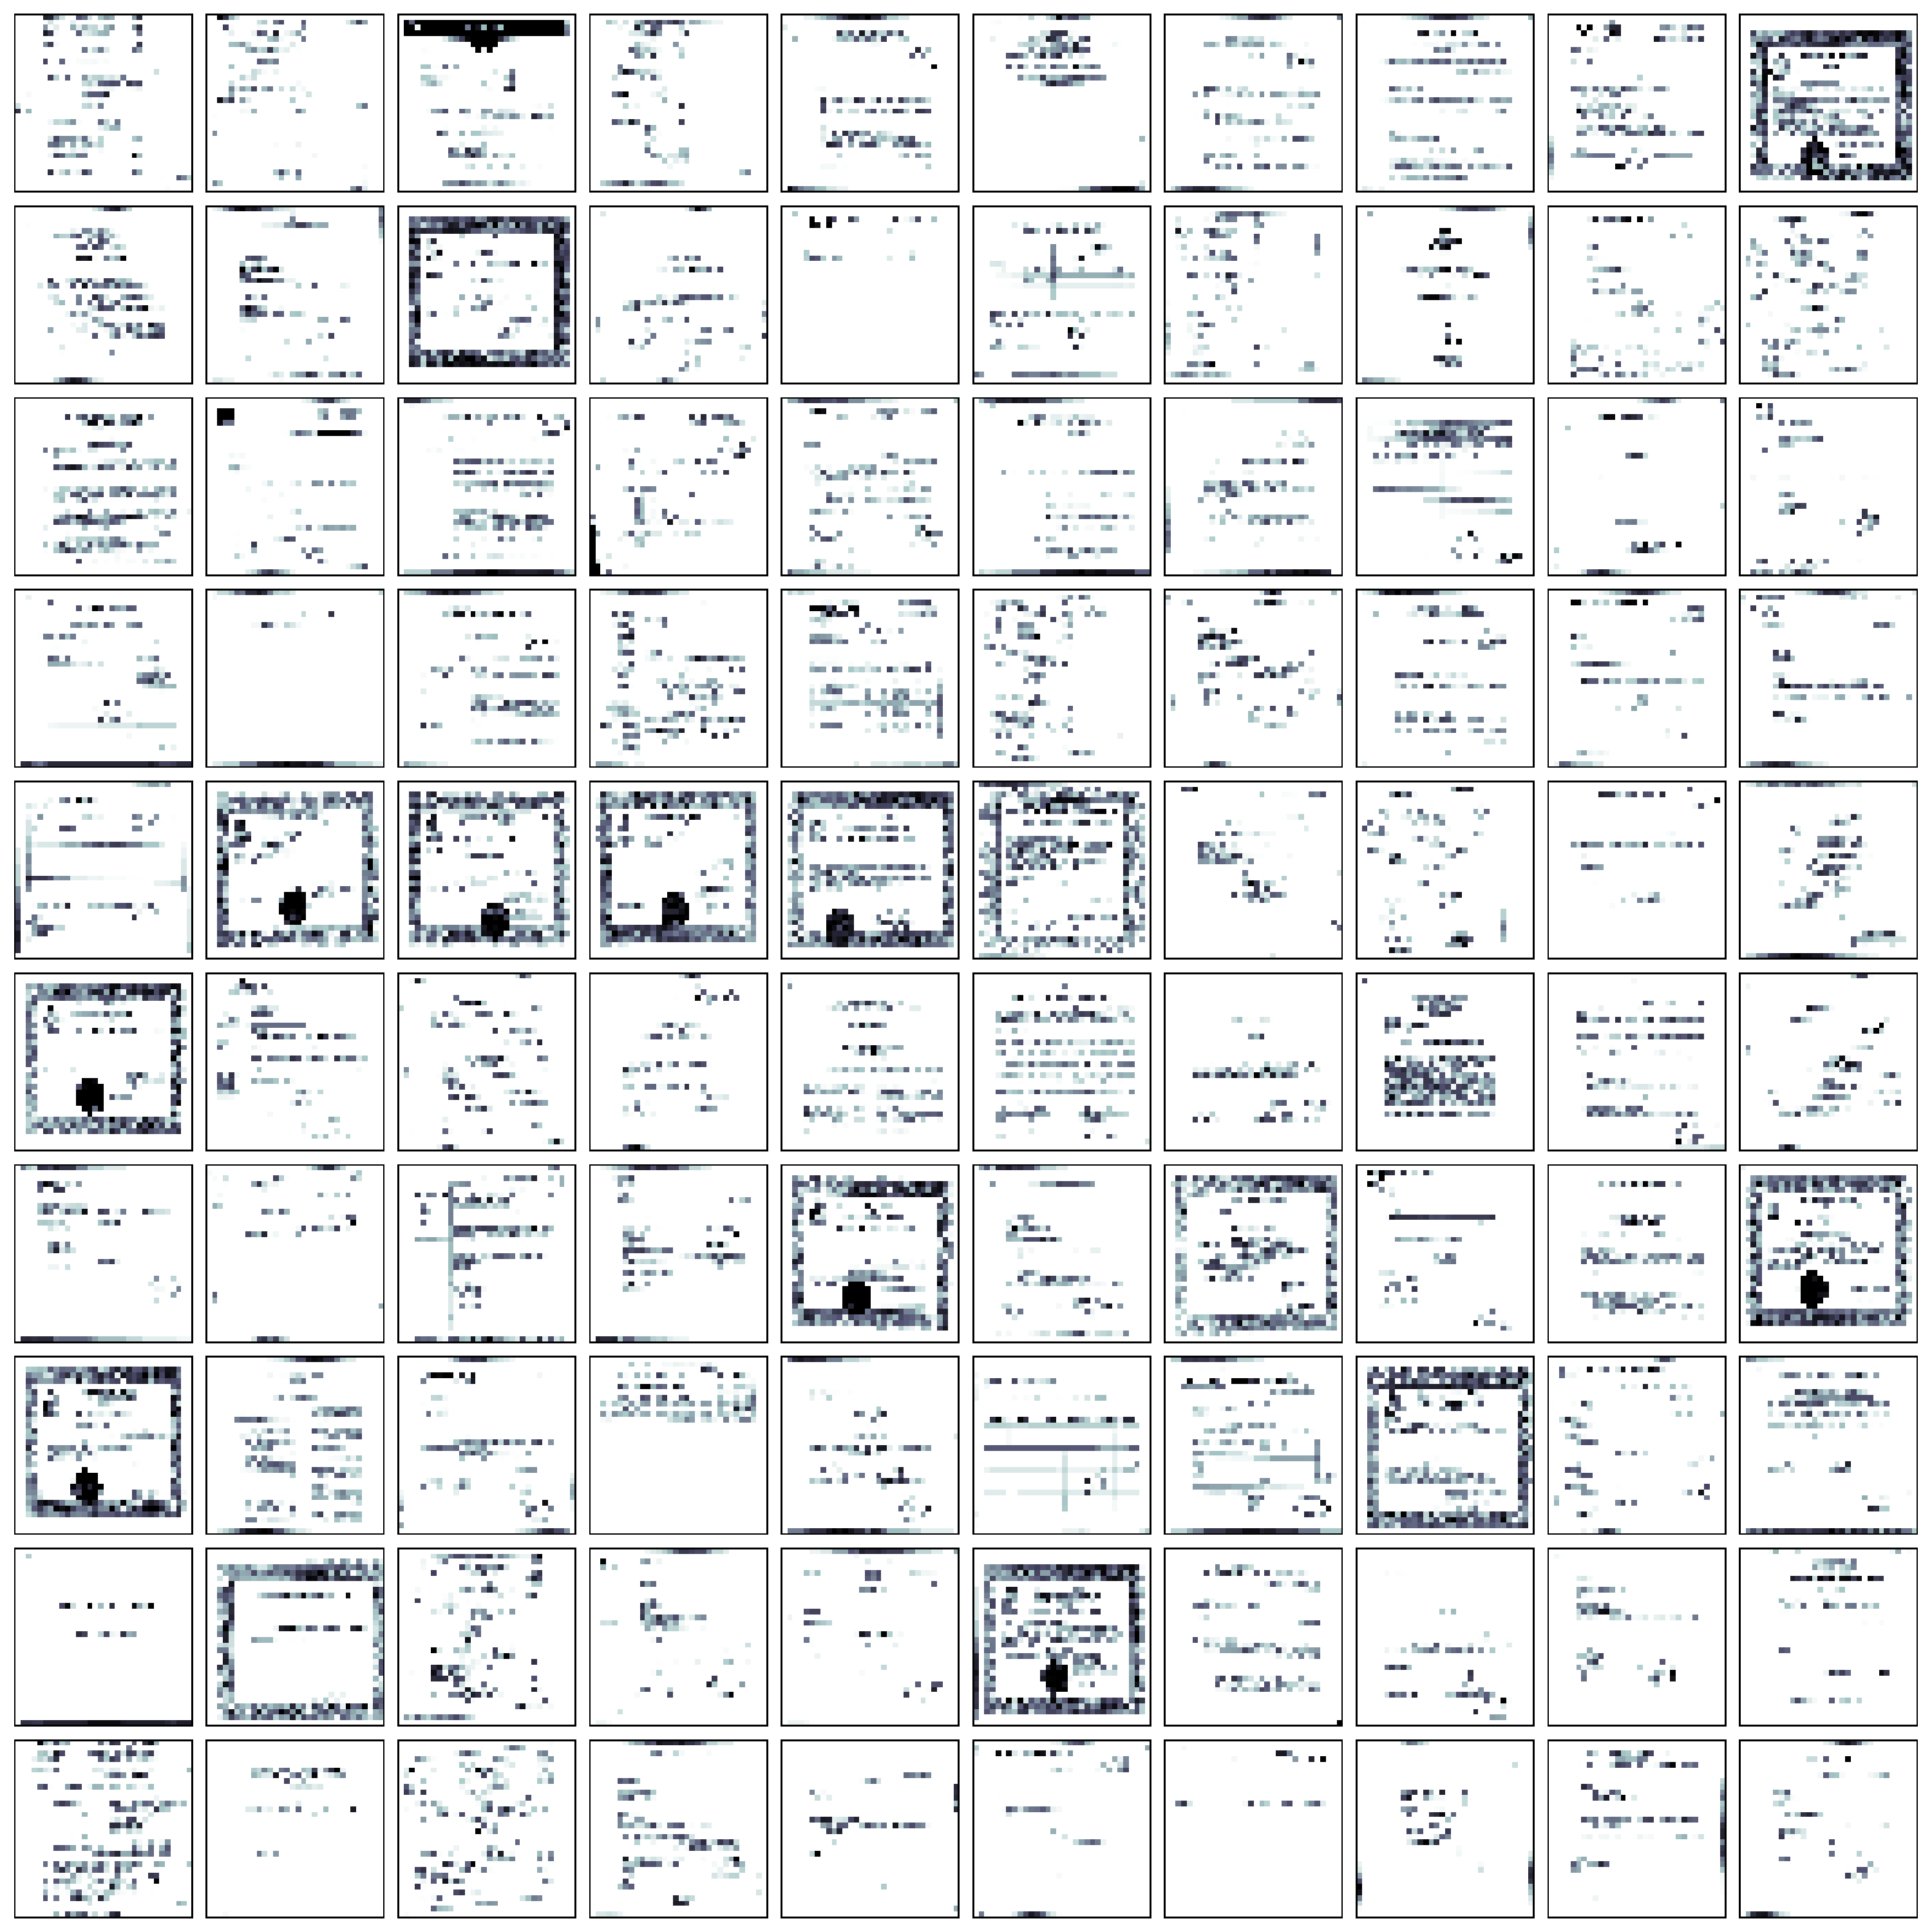
\includegraphics[width=0.4\textwidth]{images/OPTICS/32x32/preprocessed_docs.pdf}
    \caption{The first 100 documents of the dataset compressed to 32x32 greyscale pixels.
    }
    \label{fig:preprocessed_docs_32x32}
\end{figure}

The reachability distance ordered by \ac{optics} is displayed in \autoref{fig:reachability_plots}.
The resulting clusters are displayed in \autoref{fig:optics_cluster}.

% reachability plot
\begin{figure}%
    \centering
    \subfloat[\centering The reachability plot of the documents preprocessed according to \autoref{pt:32}.]{{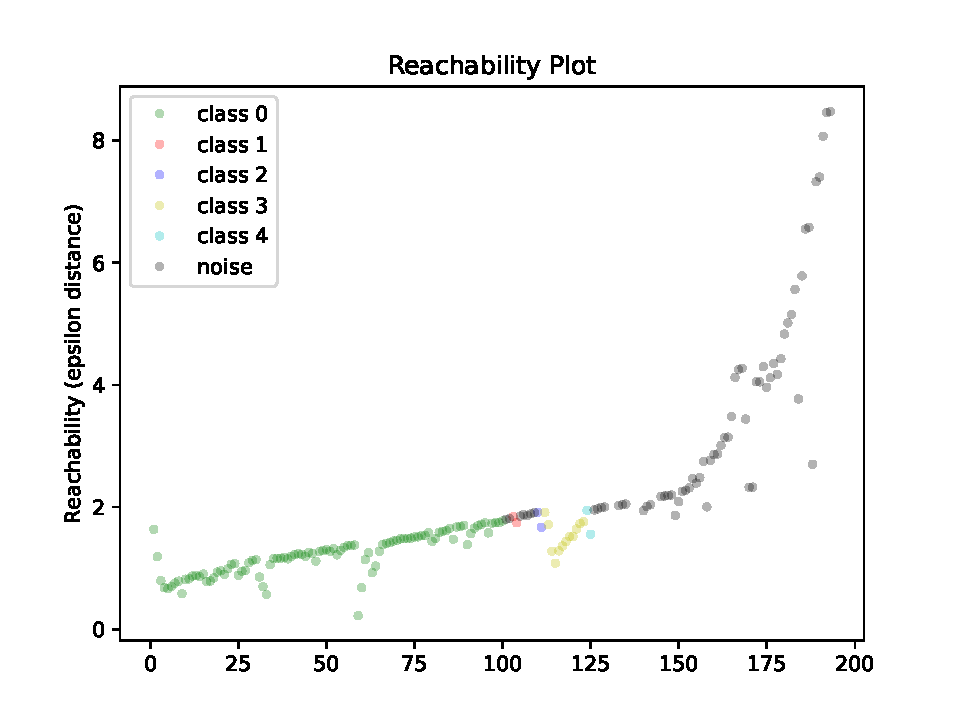
\includegraphics[width=5cm]{images/OPTICS/32x32/reachability_plot_32x32_pca_13dim.pdf} }}%
    \qquad
    \subfloat[\centering The reachability plot of the documents preprocessed according to \autoref{pt:eigendocs}.]{{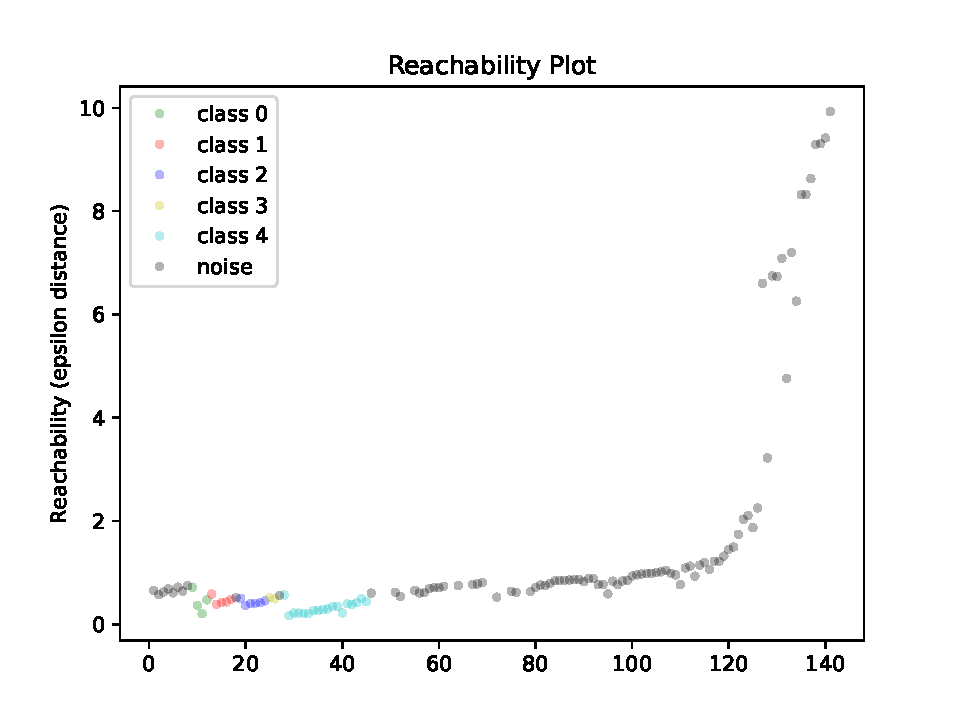
\includegraphics[width=5cm]{images/OPTICS/eigendocs/reachability_plot_13dim_eigendocs.pdf} }}%
    \caption{The plot was created using the \ac{optics} algorithm from the Python library scikit-learn.
    It shows the reachability distance of each document to its predecessor in the order list.}%
    \label{fig:reachability_plots}%
\end{figure}


\section{\acl{ui}}\label{sec:ui}

Since this work should be valuable to (German) tax offices, a basic \ac{ui} is provided.
However, the focus of this work is on the methods and not on the \ac{ui}.
The \ac{ui} is divided into two parts, the frontend and the backend.

\subsection{Backend}\label{subsec:backend}

% this work: endpoints
The framework used for the backend is \flask{}.
In this work, only the \texttt{GET} method is used.
There are multiple endpoints, which are used to retrieve data from the server:

\begin{itemize}
    \item \label{pt:docs}Documents: 
        Returns a list of documents, which best match the query.
        The query can be of type \texttt{match\_all}, which returns all documents in the database, 
        or a fuzzy full-text query, 
        or a \ac{knn} query on a certain field of the database.
        Moreover, the number and start index of the results returned can be specified.

    \item \label{pt:doc}Document: 
        Returns the document with the specified \texttt{id}.

    \item \label{pt:pdf}\ac{pdf}: 
        Returns the path to a \ac{pdf} file.
        In order to access the path information a query for a document with the specified \texttt{id} is performed.
    
    \item \label{pt:wordcloud}WordCloud: 
        Returns the bytes of a WordCloud image. 
        Depending on additional parameters, the WordCloud is either generated from one document or 
        the most similar documents to the query field, identified by \ac{knn}.

    \item \label{pt:termfrequency}Term Frequency:
        Returns the term frequency calculated for the specified document.
\end{itemize}

In order to test the endpoints during development, swagger documentation for every endpoint is provided.





\subsection{Frontend}\label{subsec:frontend}

The framework used for the frontend is \angular{}.
There are three main components, which are used to display the data:

\begin{itemize}
    \item \label{pt:home}Home: 
        The home component is used to display the results of a query.
        It consists of a search bar, which is used to enter the text query, and a list of results.
        If no text query is entered the first documents of the database, i.e. the result of a \texttt{match\_all} query, are displayed.
        The search component is shown in \autoref{fig:home_comp}.

    \item \label{pt:detail}Detail: 
        The detail component is used to display the details of a document.
        The document name and ID are located on the left side of the screen.
        Beneath the document name and ID, a button which opens the term frequency image on a new page upon pressing is located. 
        Moreover, the WordCloud of the document is displayed.
        The WordCloud is generated from the text of the document.
        On the right side of the screen, there is a \ac{pdf} viewer which displays the pages of the document.
        Beneath the \ac{pdf} viewer, the names and WordClouds of the most similar documents are displayed after a query for them is initiated by the user.
        The detail component is shown in \autoref{fig:detail_comp}.

    \item \label{pt:topic}Topic: 
        The topic component is used to display the topics of the documents.
        The topics are generated by \texttt{top2vec}.
        The topic component is shown in \autoref{fig:top2vec_topic_comp}.
\end{itemize}


\begin{figure}[htp] % htp = hier (h), top (t), oder auf einer eigenen Seite (p).
    \centering
    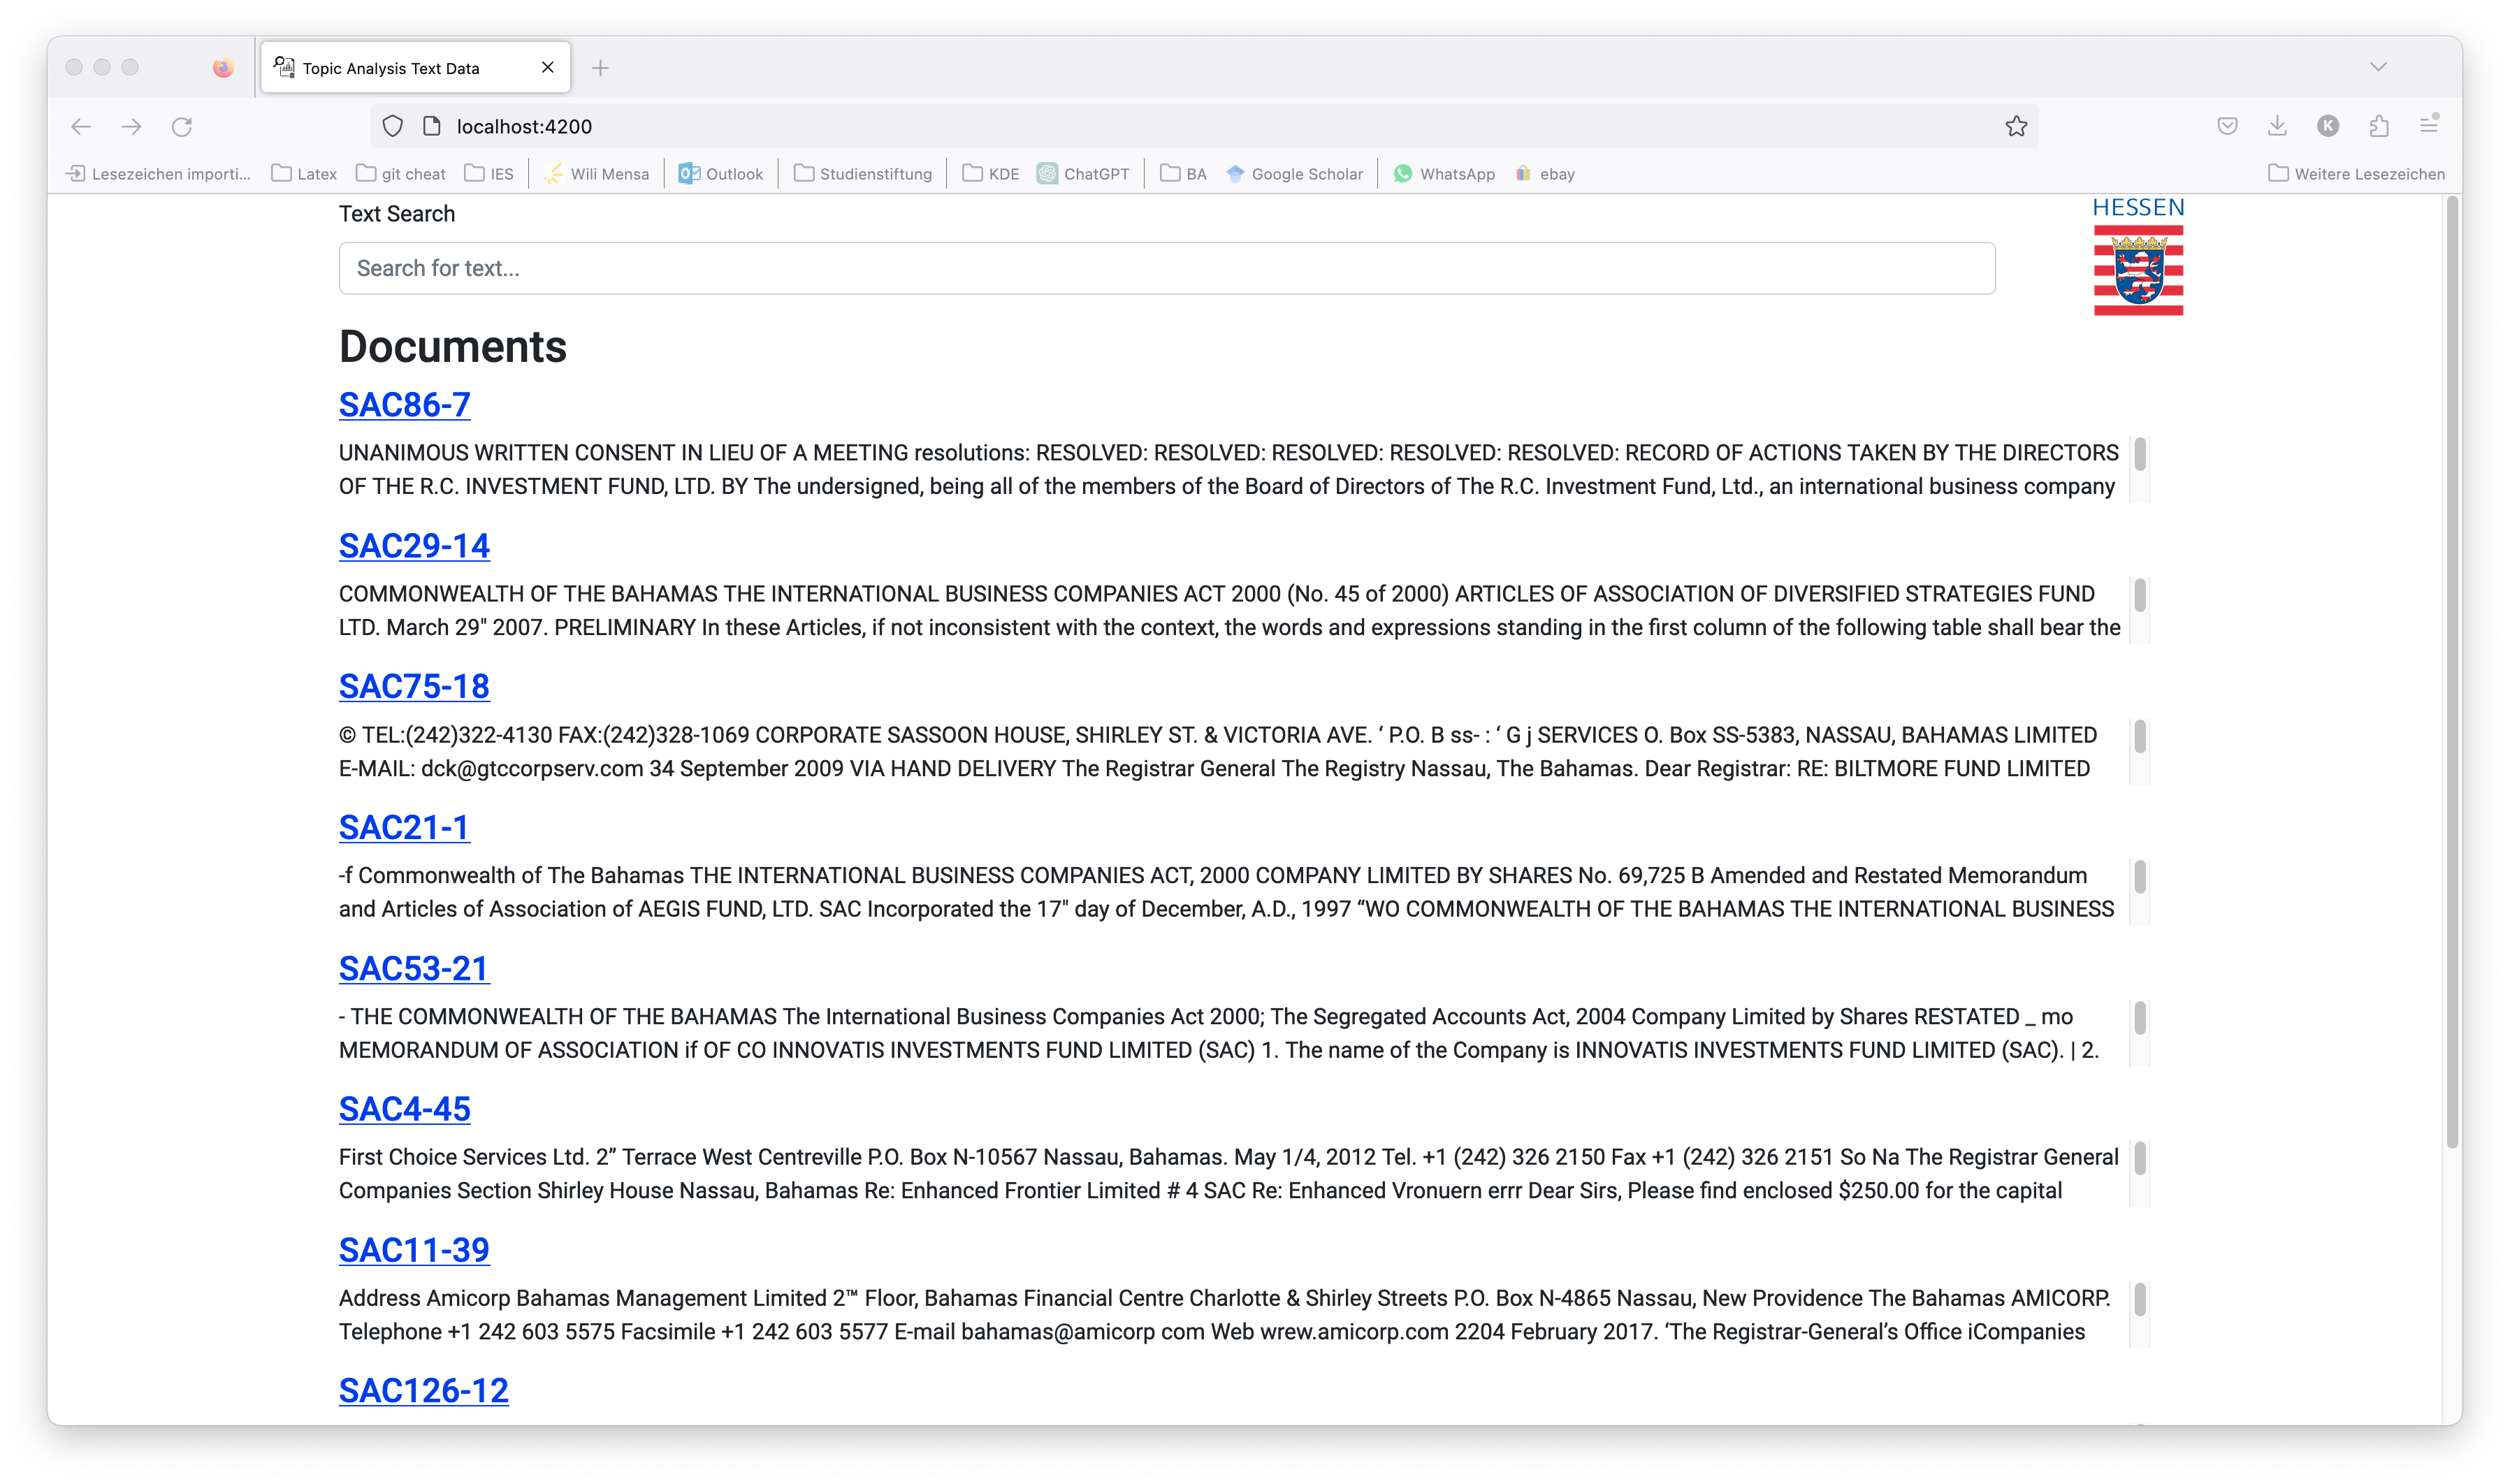
\includegraphics[width=0.7\textwidth]{images/UI/Home_component.png}
    \caption{Home component of the frontend.
    The search bar is used to enter the text query.
    The results of the query are displayed below the search bar.
    }
    \label{fig:home_comp}
\end{figure}


\begin{figure}[htp] % htp = hier (h), top (t), oder auf einer eigenen Seite (p).
    \centering
    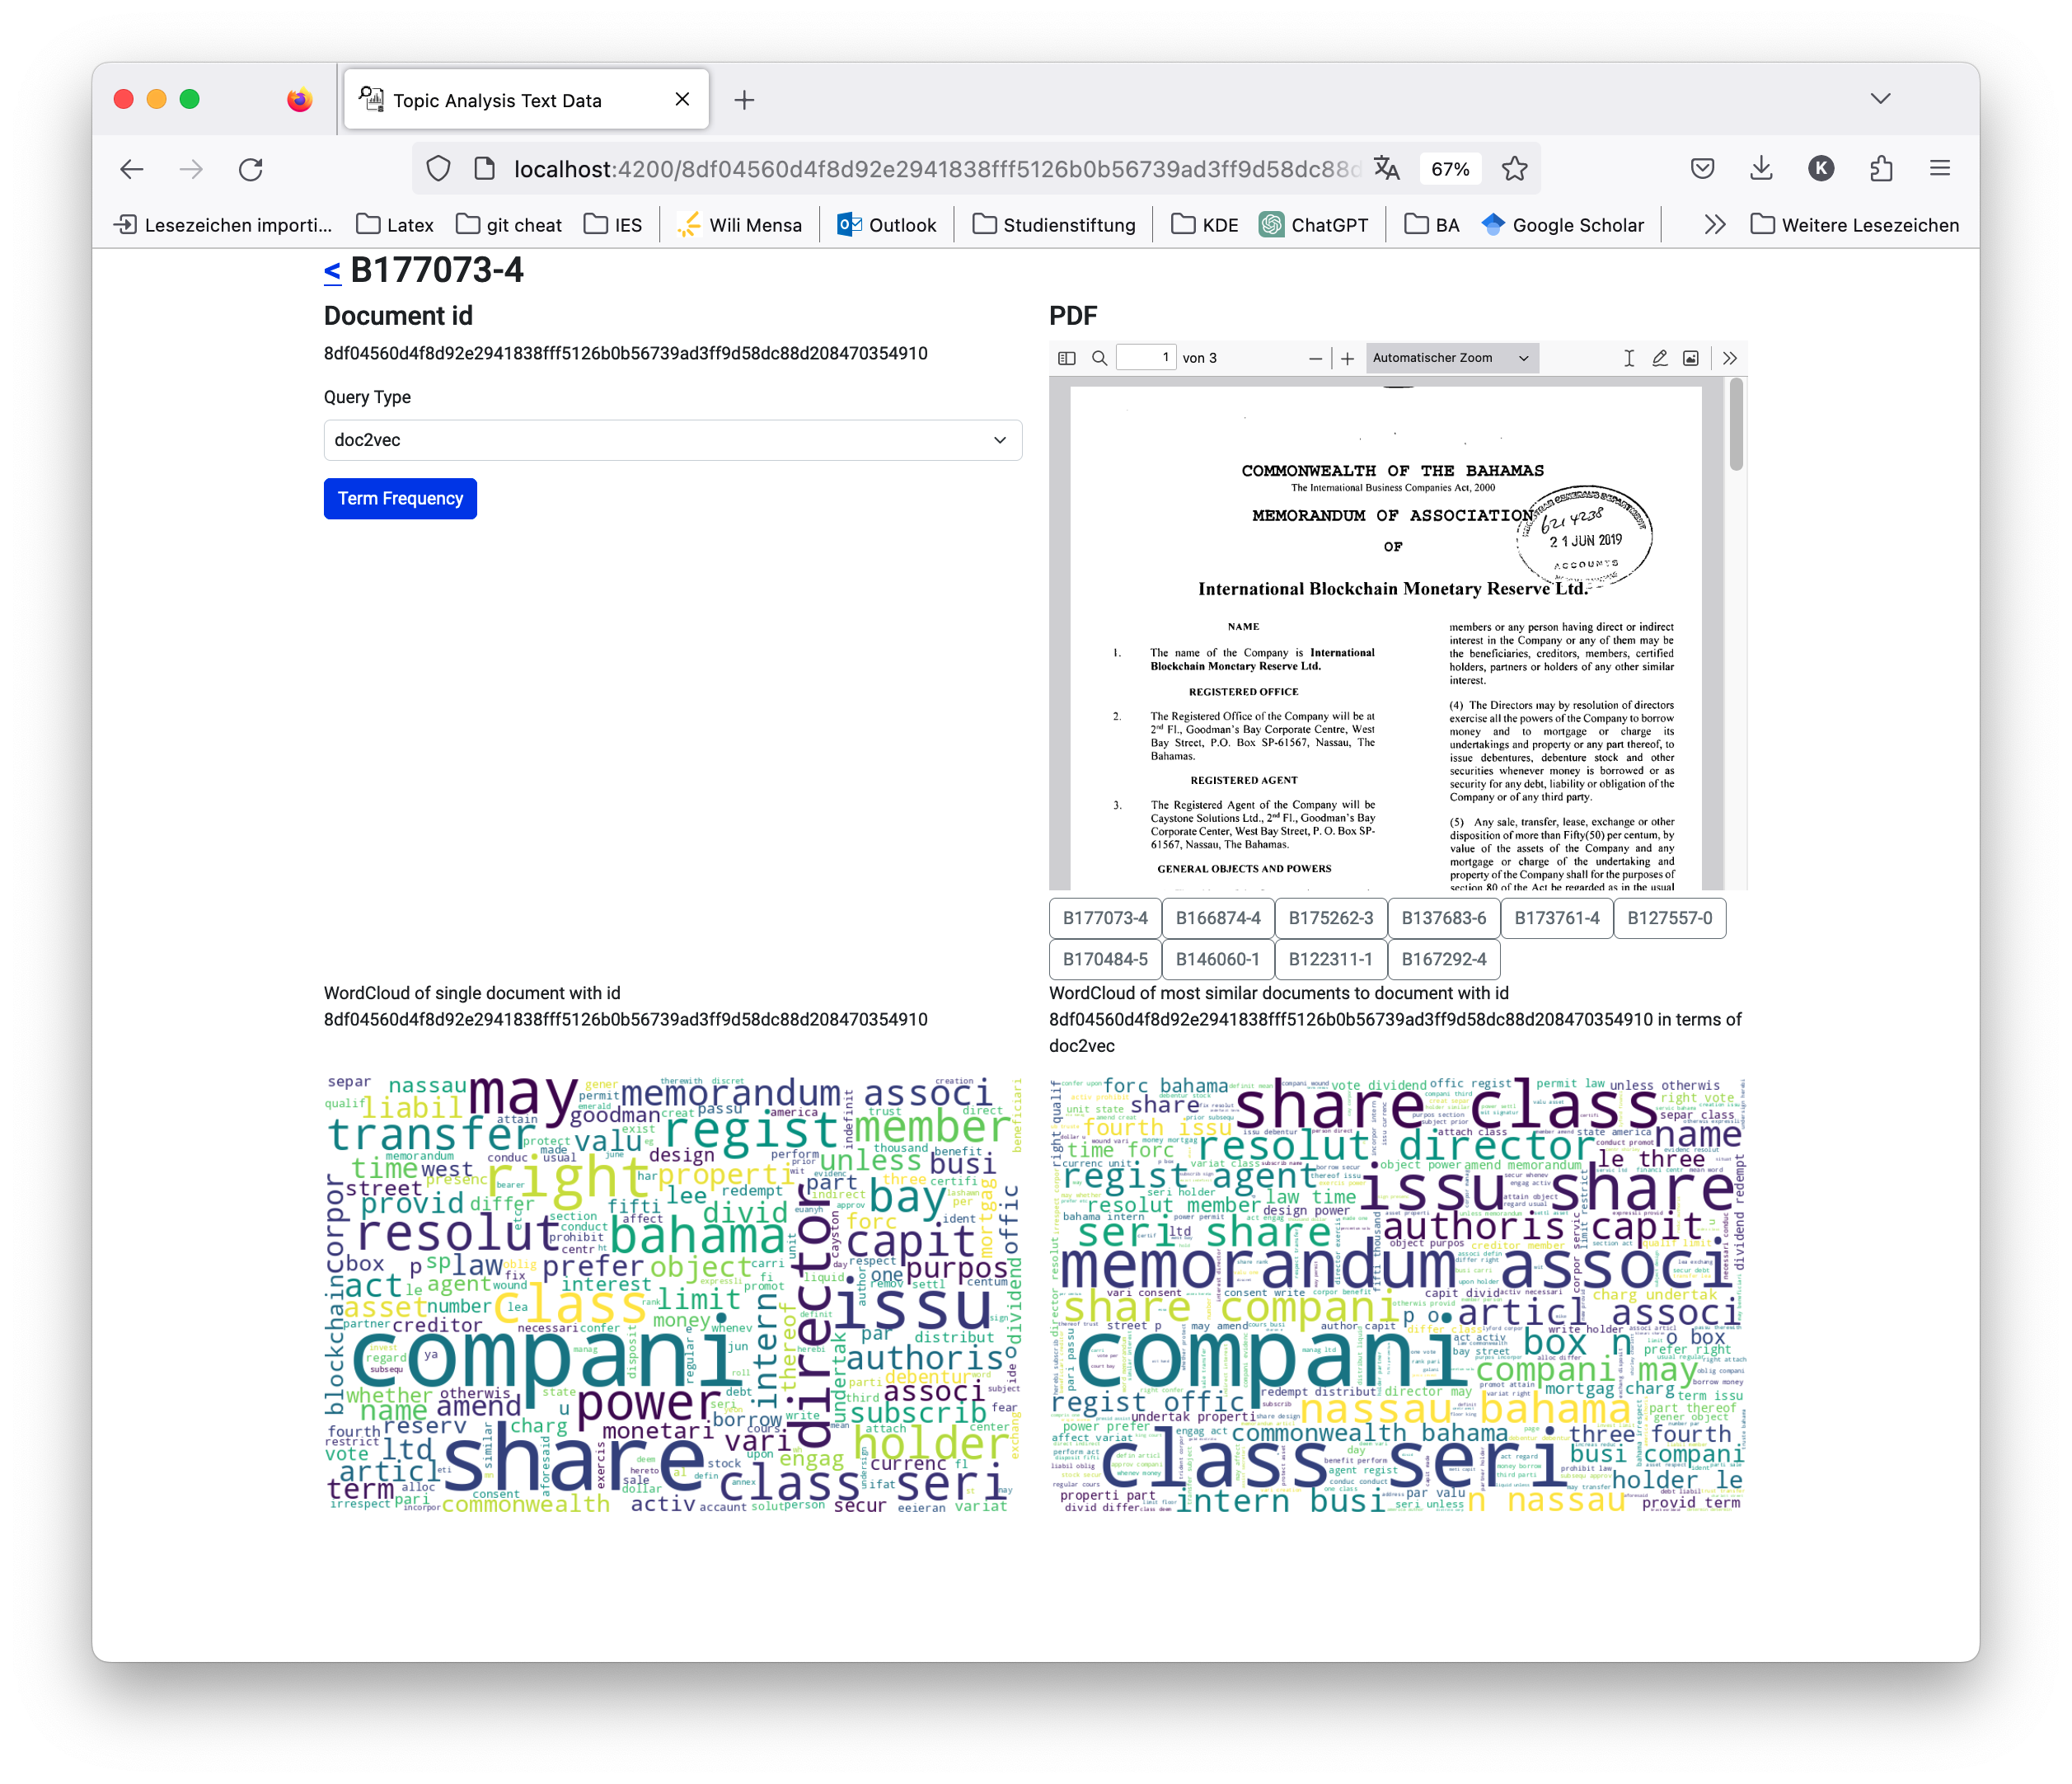
\includegraphics[width=0.7\textwidth]{images/UI/Home_detail.png}
    \caption{Detail component of the frontend.
    The chosen document is displayed, as well as its most similar documents in the database.
    WordClouds of the document and the most similar documents are displayed.
    }
    \label{fig:detail_comp}
\end{figure}


\begin{figure}[htp] % htp = hier (h), top (t), oder auf einer eigenen Seite (p).
    \centering
    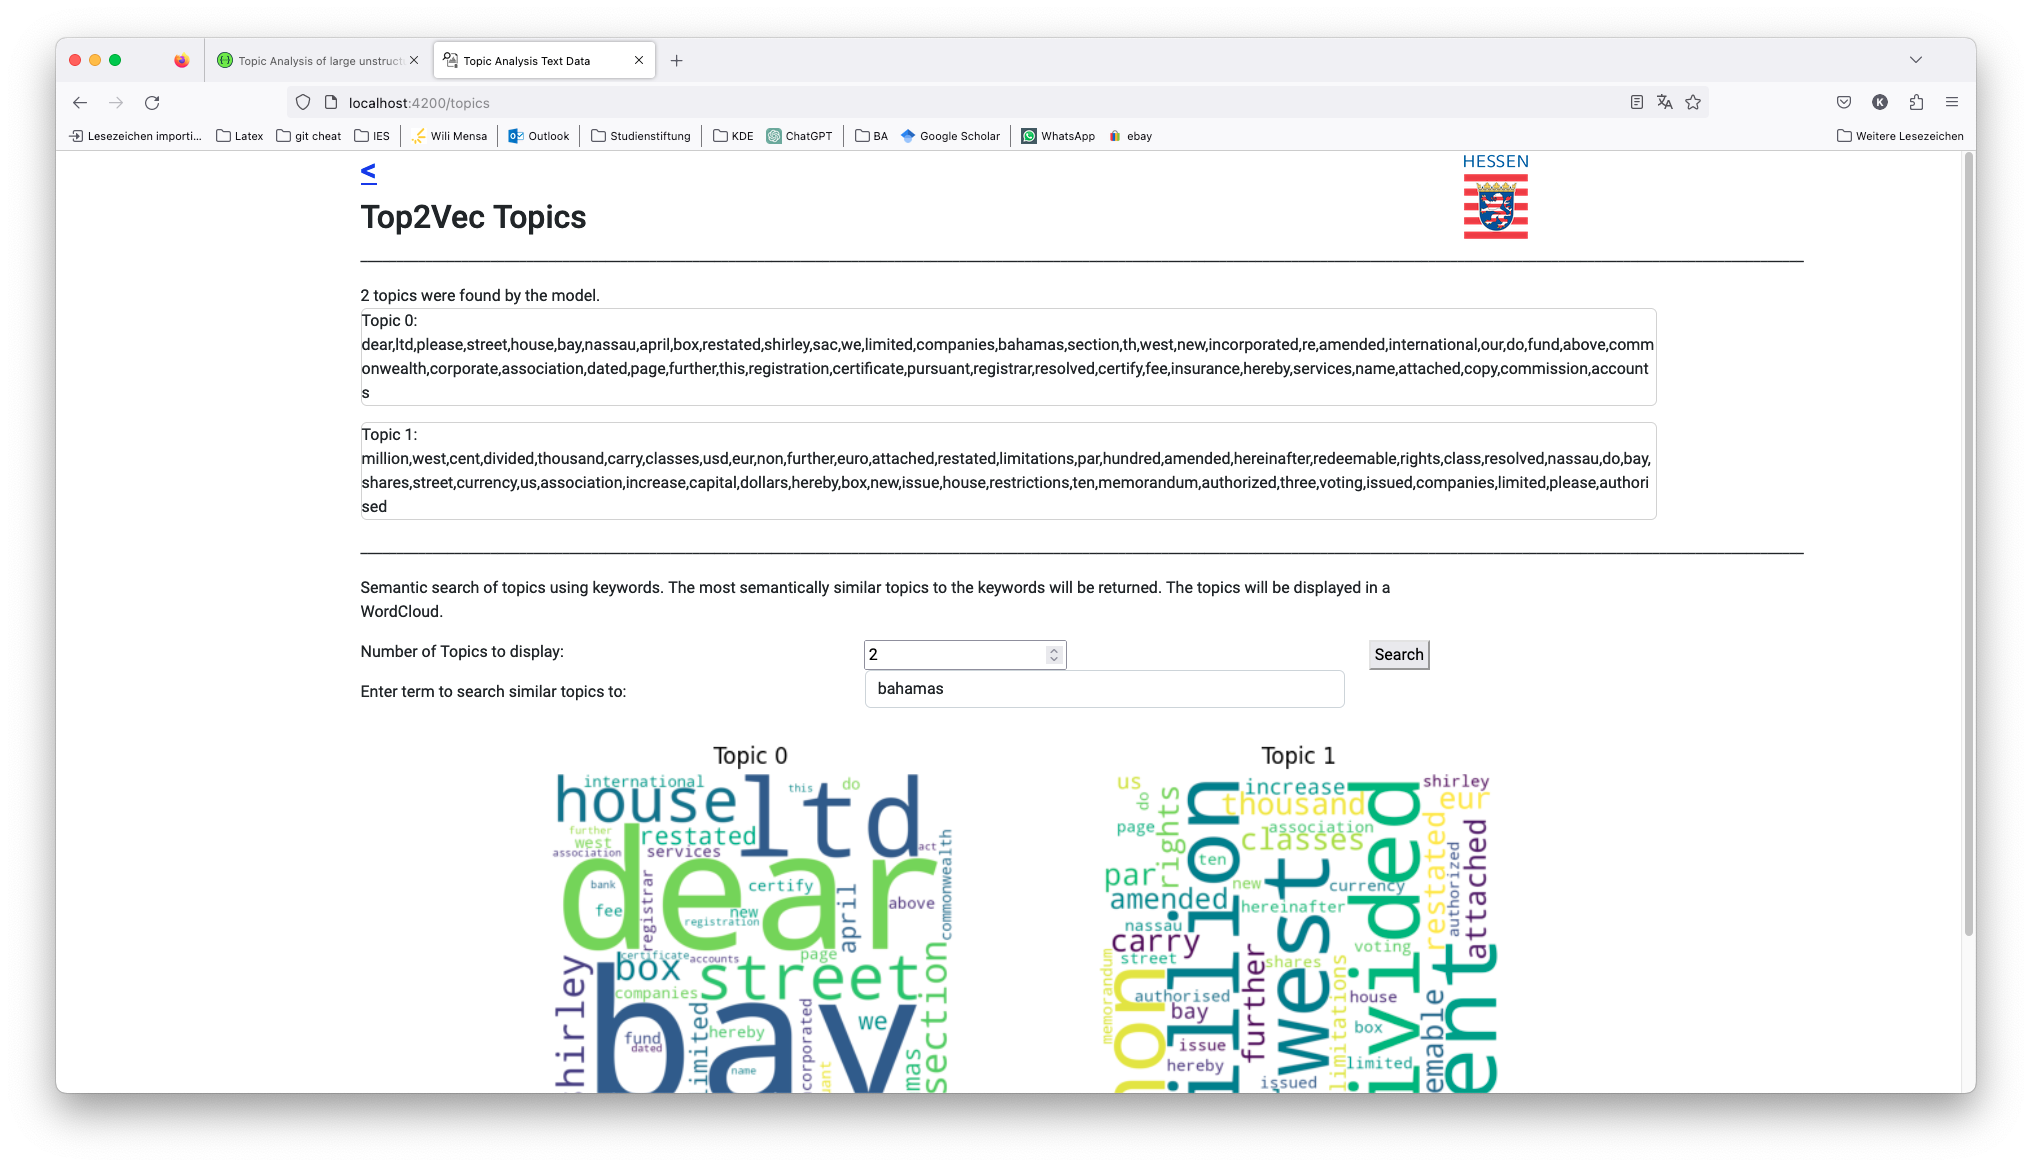
\includegraphics[width=0.7\textwidth]{images/UI/Top2Vec_Topics.png}
    \caption{Topic component of the frontend.
    }
    \label{fig:top2vec_topic_comp}
\end{figure}


To change between the components, the routes have to be defined.
The routes are defined in the \texttt{app-routing.module.ts} file, as shown in \autoref{lst:angular_routing}.

\begin{listing}[htp]
    \begin{minted}{typescript}
        const routes: Routes = [
            { path: ':id', component: DocumentDetailComponent},
            { path: '', component: HomeComponent},
          ];
    \end{minted}
    \caption{Definition of routes in \angular{} in the app-routing.module.ts.
    }
    \label{lst:angular_routing}
\end{listing}


\section{Trade-off between memory and query time}\label{sec:trade-off}
    \chapter{Evaluation}\label{ch:evaluation}
Parameters of models
\section{Similarity measurements}\label{sec:evaluation-sim-measurements}

According to \citeauthor{HfsentTrans2019}, the similarity measurements discussed above obtained roughly the same results in their experiments \cite{HfsentTrans2019}.   


\subsection{\eigendocs{}}\label{subsec:evaluation-eigendocs}
% number of components
In order to determine the optimal number of components used for \eigendocs{} the cumulative explained variance and the reconstruction error were plotted 
as displayed in \autoref{fig:det_n_comp} from \autoref{subsec:eigenface}.
The first plot indicated that 90\% of the variance is explained by 95 components.
Usually, that would have been the number of dimensions of the subspace onto which the documents would have been projected.
However, when working with cluster algorithms like \ac{optics} prior to this step, the number of dimensions should be reduced even further to achieve valid clusters.
Therefore the second approach was used.
The second plot showed the reconstruction error with respect to different numbers of components.
\textcolor{red}{"knees"} were visible at 10 and 13.
Since visual inspection accounted for the fact that the decline of the reconstruction error after 13 declined more than after 10, the number of components chosen is 13.

% results
The results of the \eigendocs{} algorithm are displayed in \autoref{fig:preprocessed_docs_eigendocs}.

\begin{figure}[htp] % htp = hier (h), top (t), oder auf einer eigenen Seite (p).
    \centering
    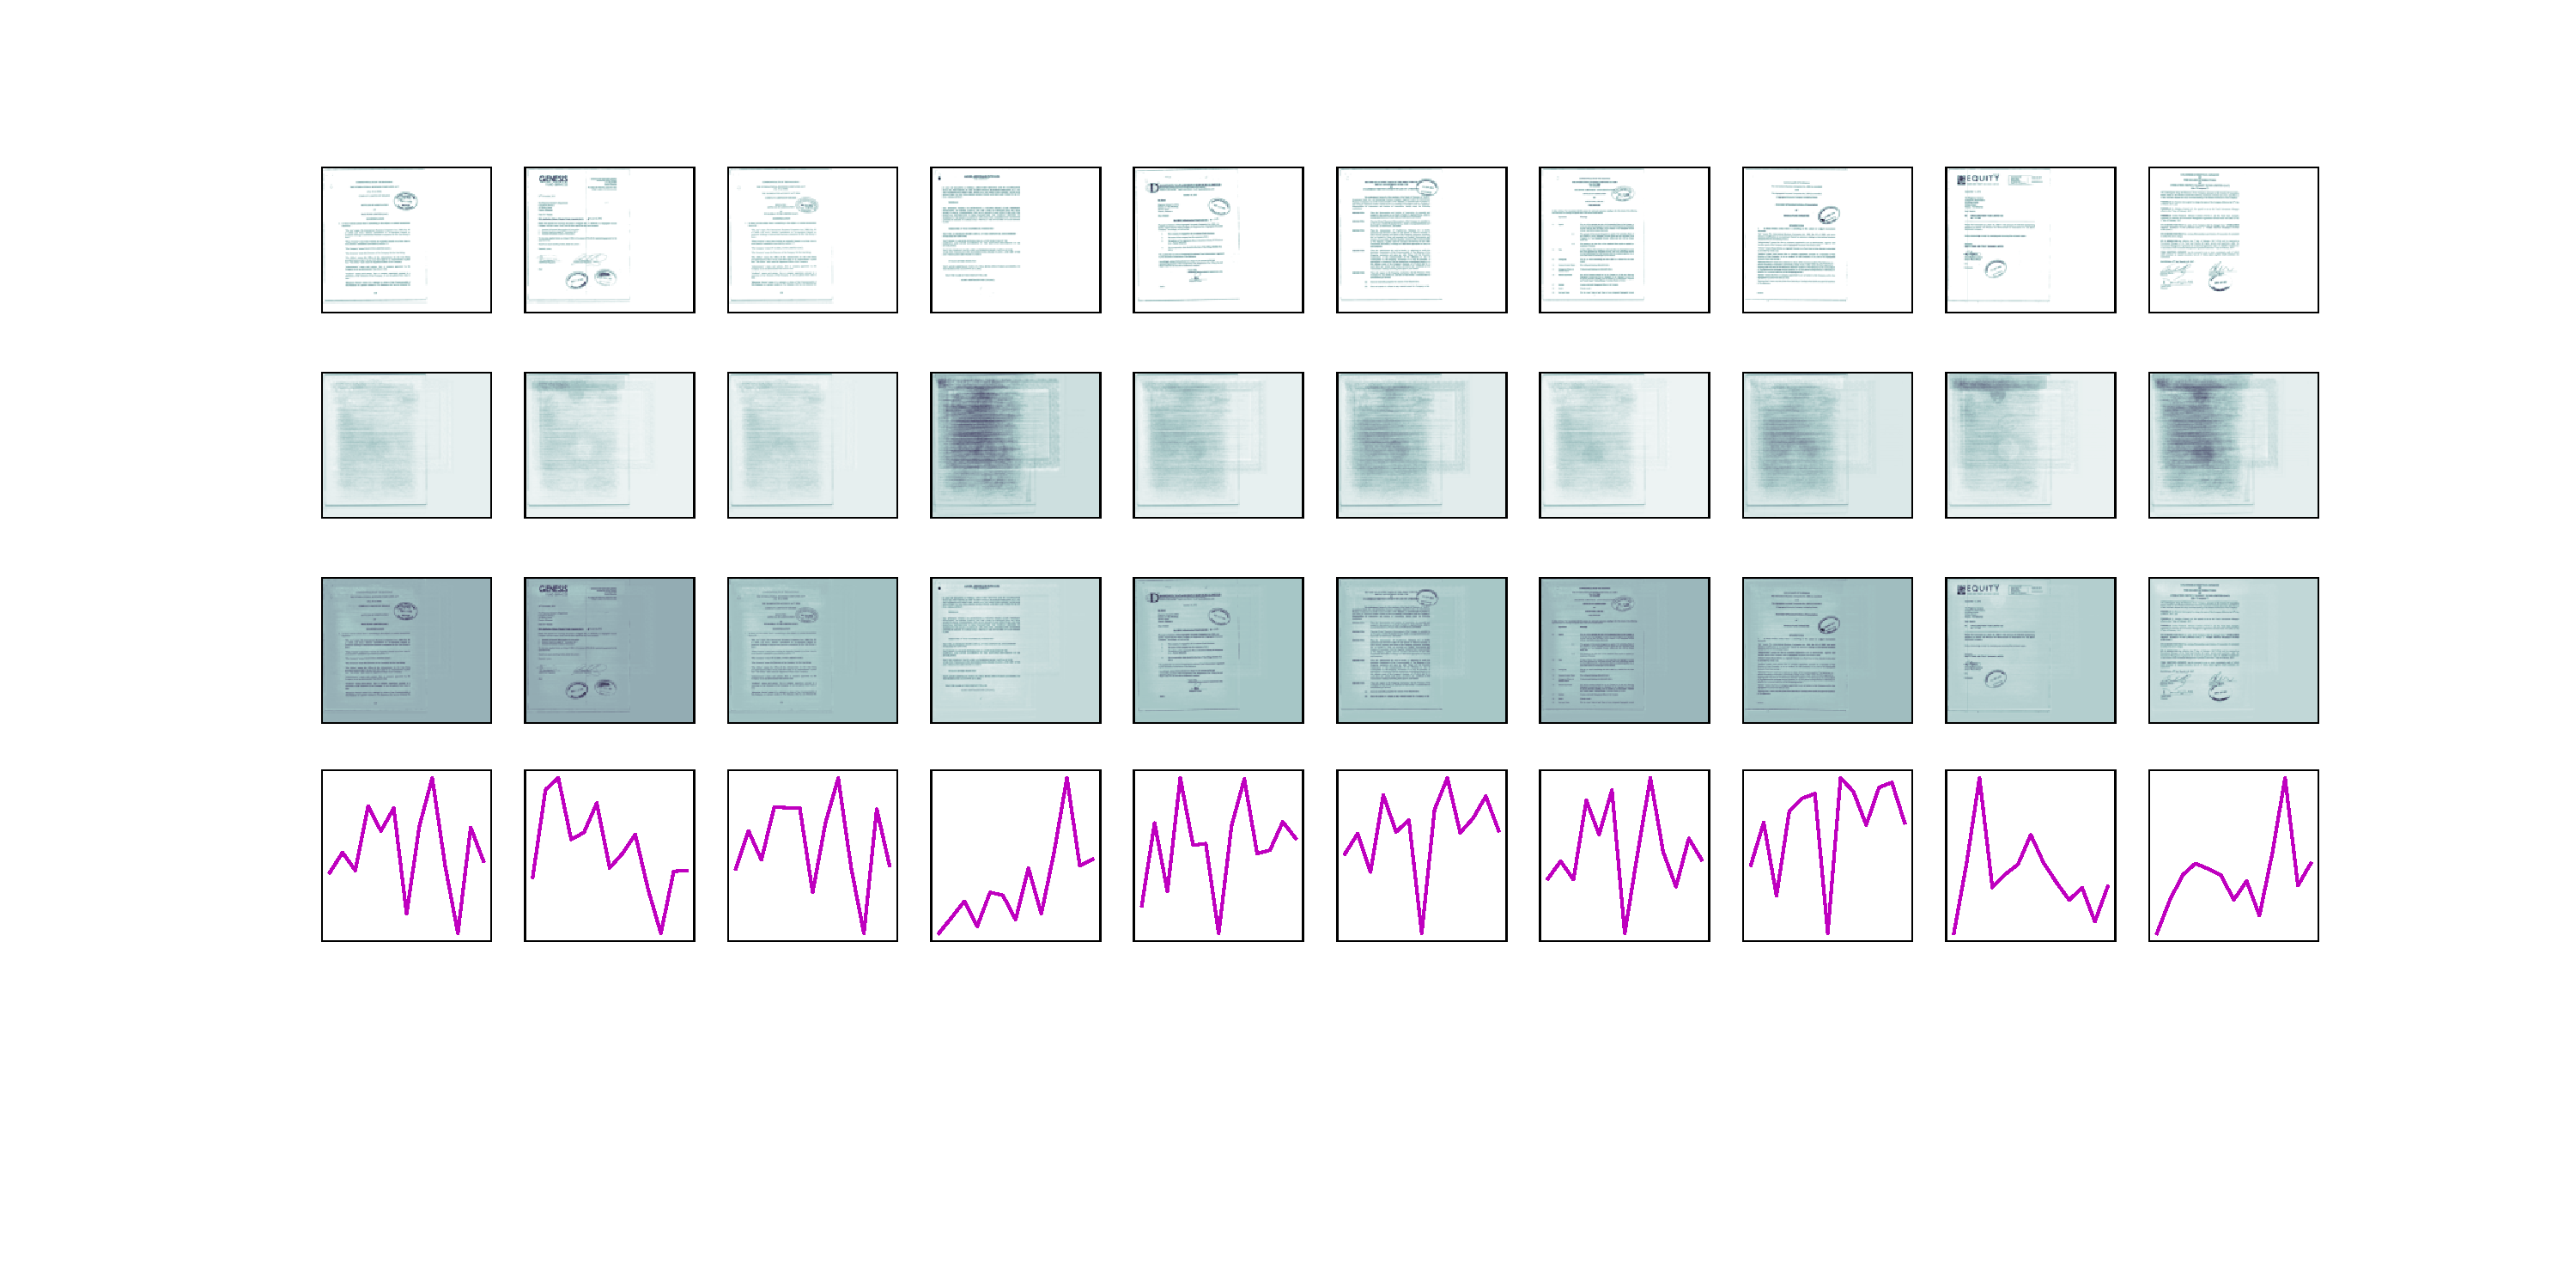
\includegraphics[width=0.7\textwidth]{images/Eigendocs/transformation/eigendocs_13dims.pdf}
    \caption{The first 10 preprocessed documents of the dataset.
    The original images are displayed in the first row.
    The second row shows the reconstructed images using the compressed images from the fourth row.
    The third row shows the reconstruction error, i.e. the difference between the reconstructed and the original image.
    The last row presents the greyscale values of the compressed 13-dimensional image as a line.
    }
    \label{fig:preprocessed_docs_eigendocs}
\end{figure}

\section{Evaluation of \ac{ae}}\label{sec:evaluation-ae}

% architecture
In order to determine, which architecture for the latent/ hidden space of the \ac{ae} is the best option, 
different architectures were tested and compared in terms of \ac{rsme} and cosine similarity.
The \ac{rsme} is calculated as given in \lst{lst:impl-rsme}.
The cosine similarity is calculated as given in \lst{lst:impl-cos_sim}.
The dataset used for the evaluation is a selection of 195 documents from the Bahamas dataset.

% RSME
\begin{listing}[htp]
    \begin{minted}{python3}
        rsme = np.linalg.norm(inverse_embedding - embeddings) 
                / np.sqrt(embeddings.shape[0])
    \end{minted}
    \caption{
        Computation of the \ac{rsme} between the original and the reconstructed embedding.
    }
    \label{lst:impl-rsme}
\end{listing}

% cosine similarity
\begin{listing}[htp]
    \begin{minted}{python3}
        cos_sim = statistics.mean([np.dot(inverse_emb, embedding)
                /(np.linalg.norm(inverse_emb)*np.linalg.norm(embedding)) 
                for inverse_emb, embedding in zip(inverse_embedding, embeddings)])
    \end{minted}
    \caption{
        Computation of the cosine similarity between the original and the reconstructed embedding.
    }
    \label{lst:impl-cos_sim}
\end{listing}

The scores of different architectures are shown in \fig{fig:eval-ae-architecture}.
While most of the architectures produced similar results, one architecture stood out.
Combining 2500, 3000 and 3500 dimensions in the hidden space produced the worst \ac{rsme} results.
The best results were achieved by adding 3500-dimensional layers in the hidden space.
However, the results of the best architecture do not differ greatly from the others.

\begin{figure}[h] % htp = hier (h), top (t), oder auf einer eigenen Seite (p).
    \centering
    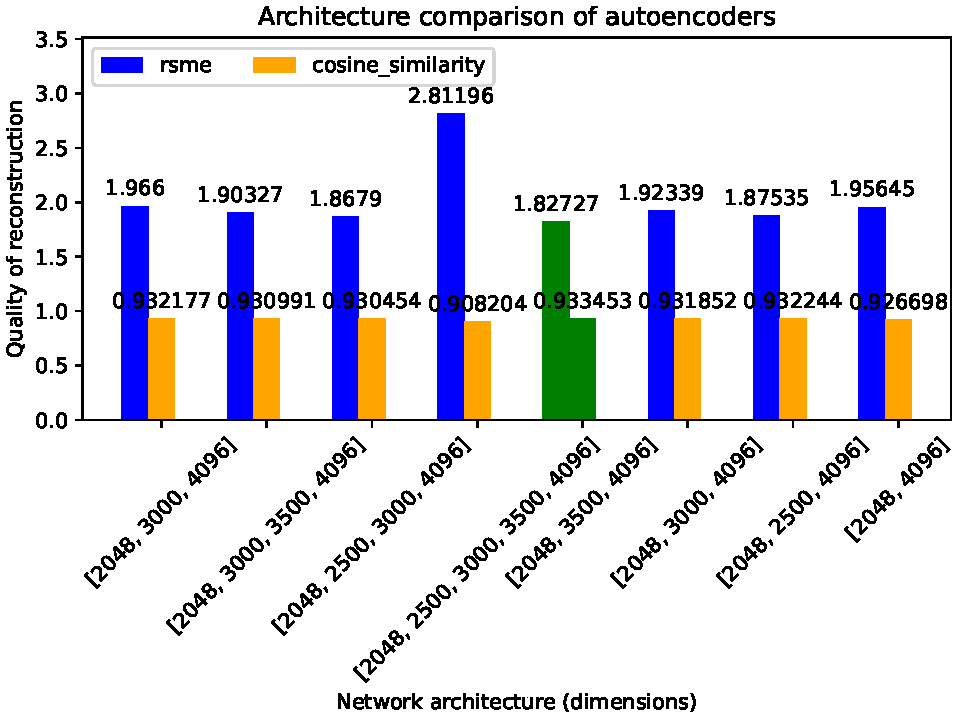
\includegraphics[width=0.7\textwidth]{images/embeddings/autoencoder/ae_score_plot.pdf}
    \caption{The effect of different \ac{ae} architectures on the reconstruction error.
    The error is measured in terms of \ac{rsme} (blue bars) and cosine similarity (yellow bars) between the original and the reconstructed image.
    The smallest \ac{rsme} and the biggest cosine similarity belong to the architecture best suitable to this task and are coloured green.
    }
    \label{fig:eval-ae-architecture}
\end{figure}

\subsection{Evaluation of \ac{optics}}\label{subsec:evaluation-OPTICS}

\textcolor{red}{TODO: compare preprocessing results}


% preprocessed images
\begin{figure}[htp] % htp = hier (h), top (t), oder auf einer eigenen Seite (p).
    \centering
    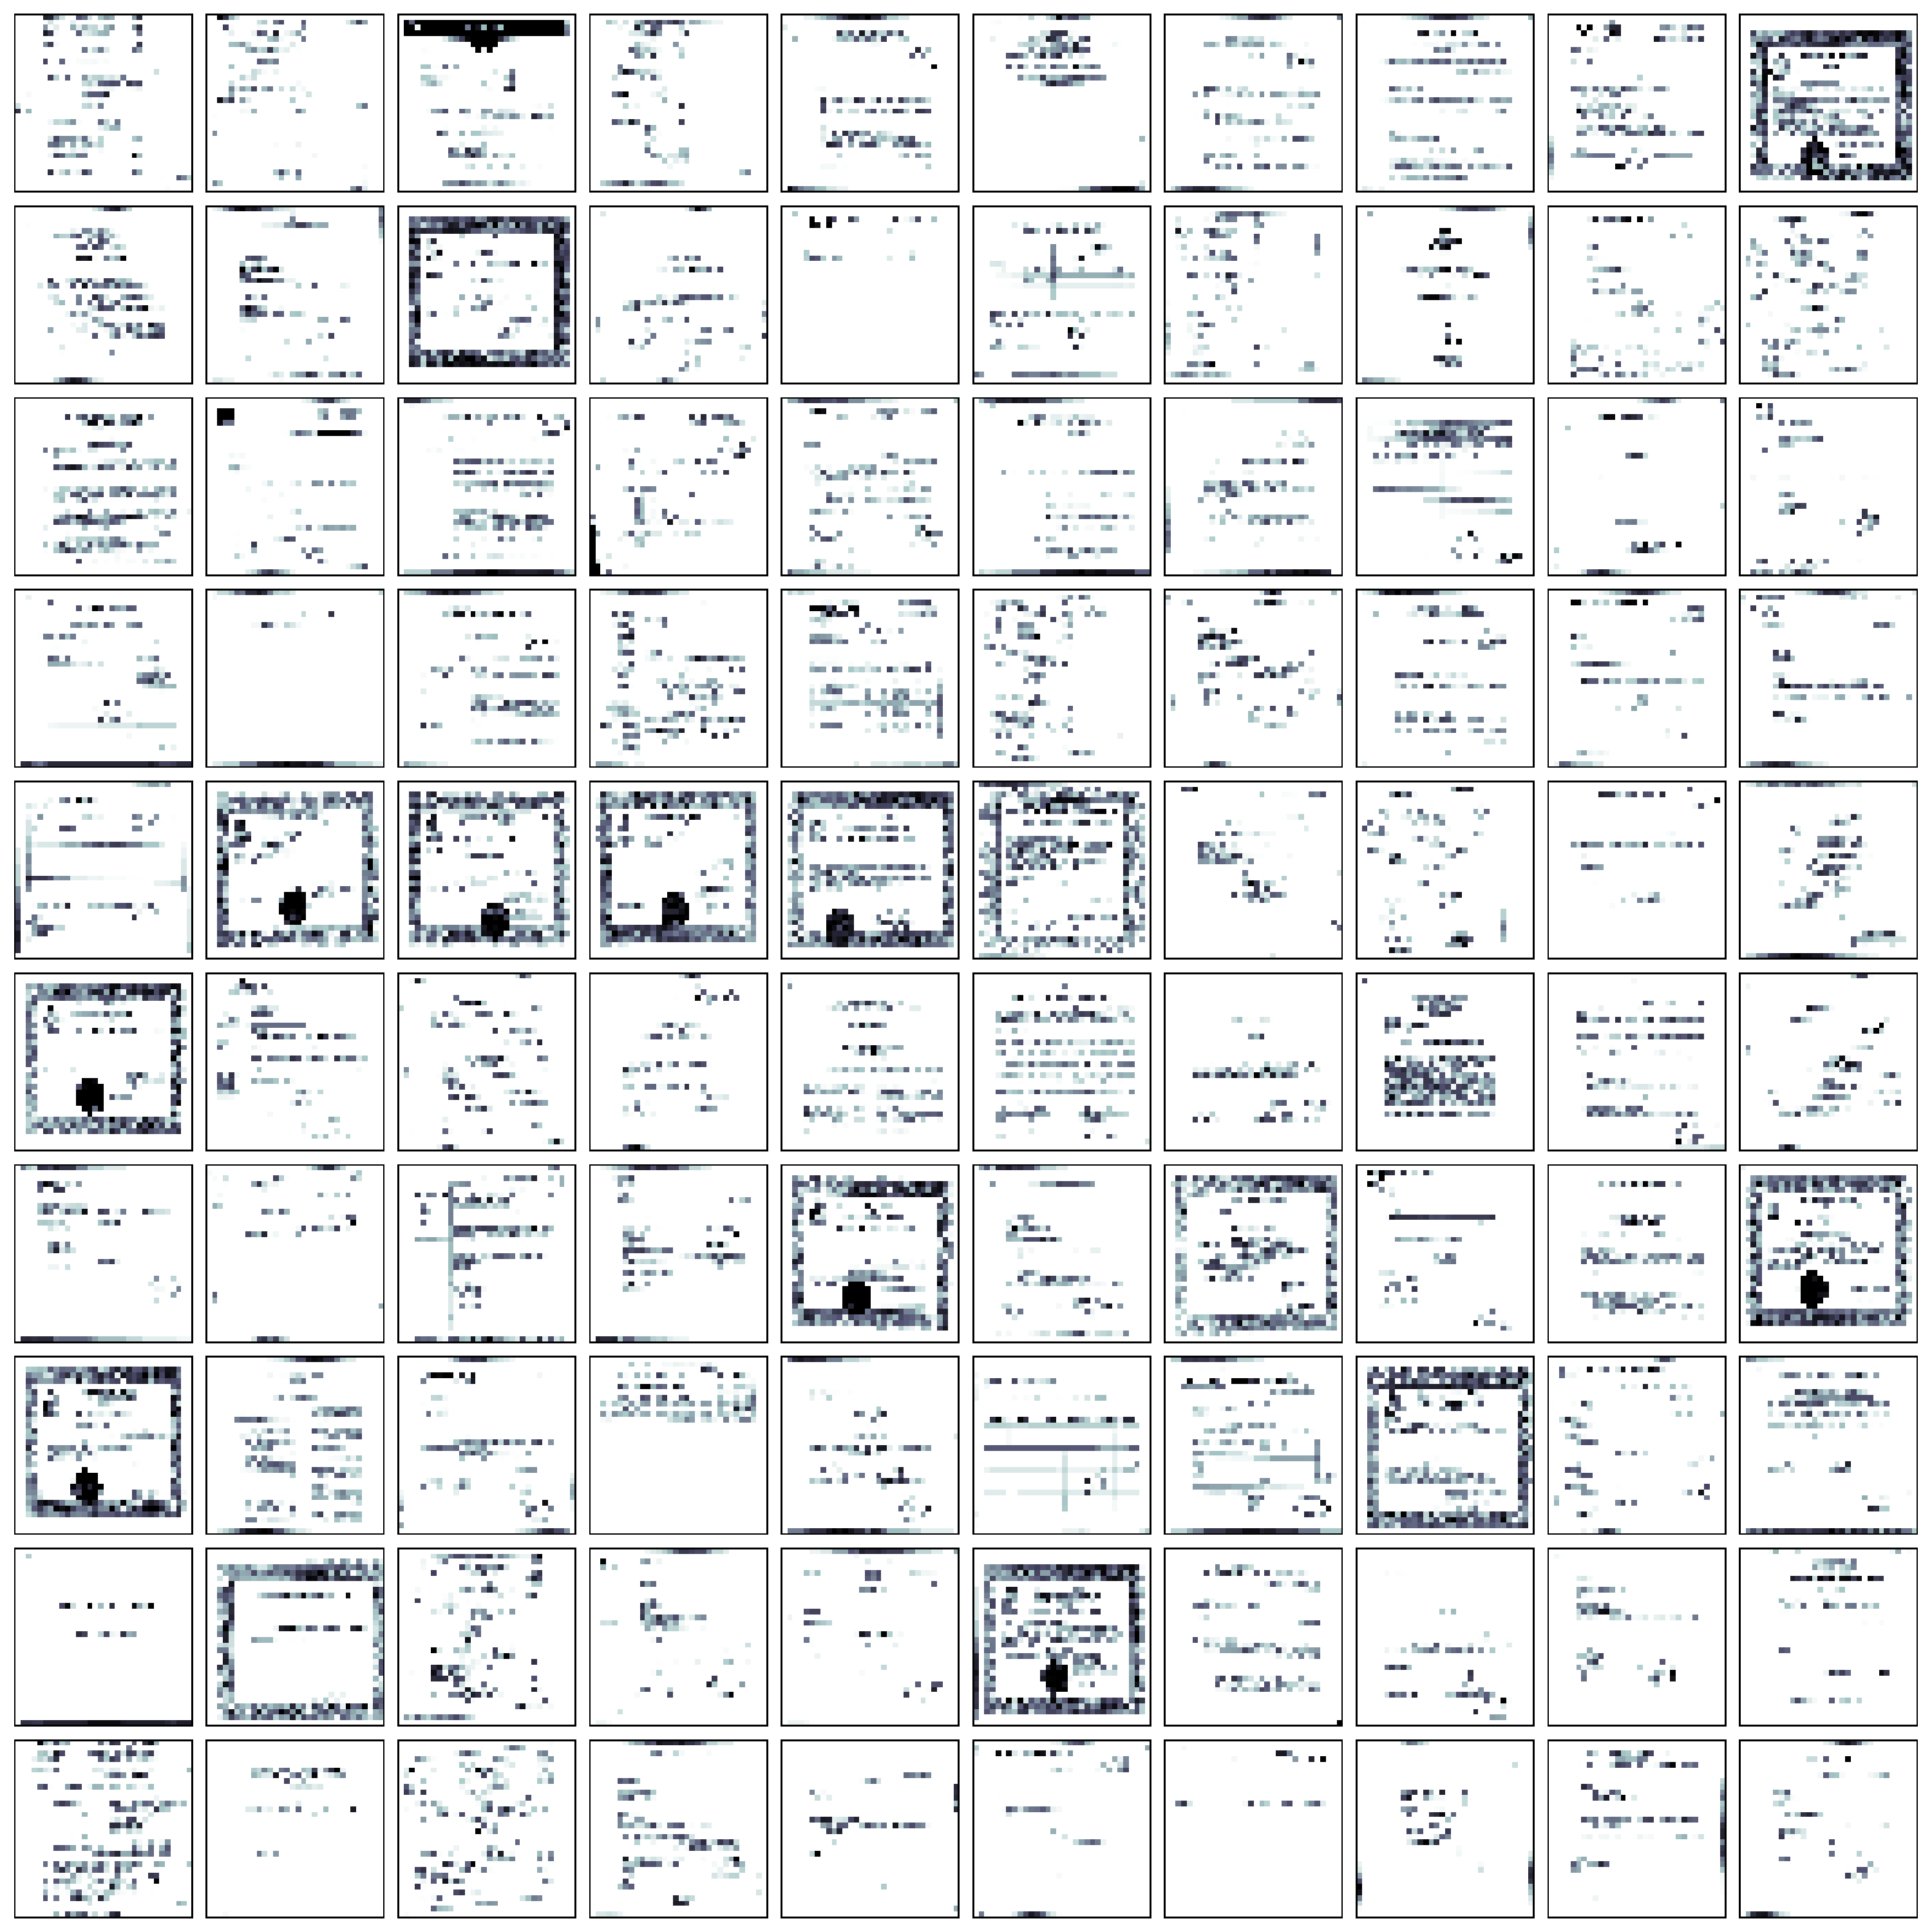
\includegraphics[width=0.5\textwidth]{images/OPTICS/32x32/preprocessed_docs.pdf}
    \caption{The first 100 preprocessed documents of the dataset.
    They were preprocessed in order to have the same characteristics as the images used in \cite{OPTICS1999}.
    The images were preprocessed as discussed in \autoref{pt:32} to 32x32 greyscale pixels, which drastically reduced the quality of the images.
    }
    \label{fig:preprocessed_docs_32x32}
\end{figure}




% OPTIC cluster results
\begin{figure}%
    \centering
    \subfloat[\centering The clusters identified by \ac{optics} of the documents preprocessed according to \autoref{pt:32}.]{{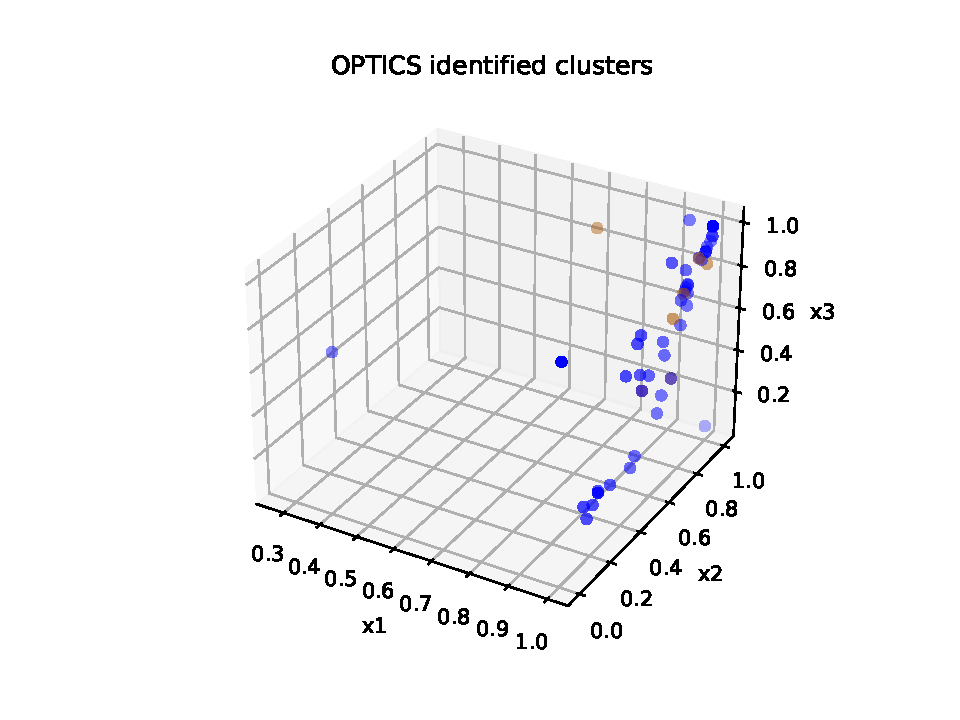
\includegraphics[width=5cm]{images/OPTICS/32x32/OPTICS_cluster_32x32.pdf} }}%
    \qquad
    \subfloat[\centering The clusters identified by \ac{optics} of the documents preprocessed according to \autoref{pt:eigendocs}.]{{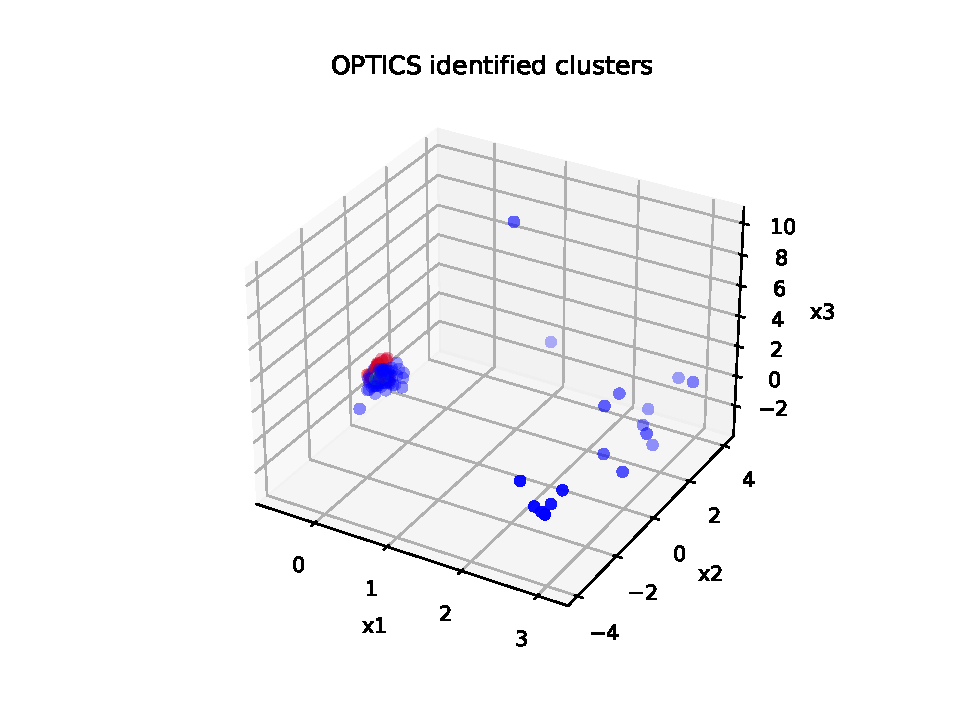
\includegraphics[width=5cm]{images/OPTICS/eigendocs/OPTICS_cluster_eigendocs.pdf} }}%
    \caption{The clusters were extracted from the respective reachability plot in \autoref{fig:reachability_plots}.
    The blue points are noise points, whereas any other colour denotes a cluster.}%
    \label{fig:optics_cluster}%
\end{figure}

\section{Evaluation of database}\label{subsec:evaluation-db}

According to \cite{flask_book2018}, \ac{sql} databases are a good choice for efficiently storing structured data.
This is because their paradigm \acs{acid}, i.e. \acl{acid}, provides high reliability.
\ac{nosql} databases, on the other hand, are more flexible and can be used to store unstructured data \cite{flask_book2018}.
They do not require a predefined schema and can therefore accept documents of arbitrary structure \cite{flask2018}.

Usually, \ac{nosql} databases do not offer services such as \texttt{JOIN} \cite{flask2018}.
According to \citeauthor{flask2018}, \ac{nosql} databases make a tradeoff between storage and speed, as well as a tradeoff between consistency and availability.
\ac{nosql} databases are said to outperform out-of-the-box \ac{sql} databases \cite{flask2018}.

A document store database can be used if the primary goal is to write fast rather than write save \cite{flask2018}.

\section{Evaluation of \acs{tfidf}}\label{sec:evaluation-tfidf}

The main obstacle to overcome was the high dimensionality of the \ac{tfidf} embeddings.
Hence, the goal of the parameter selection was to find a way to reduce the dimensionality of the vocabulary to the maximum vector dimensionality of \databaseName{}.
However, the quality of the embeddings should not decline too much.

% parameter selection
The choice of the preprocessor was investigated with regard to the goal of minimizing the vocabulary size.
Both the default and custom preprocessor were tested on a data corpus of 195 documents with regard to the vocabulary (size) and the result of preprocessing.
While the default preprocessor had a vocabulary size of 1641, the custom preprocessor had a size of 1906.
The custom preprocessor was chosen because it had a smaller vocabulary size and TODO: vocab of custom.

% two fields in db
Initially, there should have been two different \ac{tfidf} models.
The first one should have been used to obtain documents which are similar to the query document.
Therefore, terms which occur only once in the corpus should have been removed from the vocabulary.
The second approach should have been used to obtain specific documents from the corpus.
Hence, the vocabulary should consist of very document-specific terms and thus, \texttt{max\_df} would have been relatively low, to omit terms that occur in many documents.
However, the restrictions imposed by the database implementation made it impossible to explore many parameter ranges.
Therefore, only one \ac{tfidf} model was used in the end, whose parameters \texttt{min\_df} and \texttt{max\_df} were set to values which kept the vocabulary and thus,
the dimensionality of the embeddings reasonably small.

\section{Evaluation of \ac{d2v}}\label{sec:evaluation-doc2vec}

Since no labelled data is available, the evaluation of the \ac{d2v} embeddings is limited.
Therefore, the \ac{d2v} embeddings are evaluated by comparing them to other embeddings.
The \ac{d2v} model is not tuned in terms of hyperparameter selection,
but the default settings are used since there is no way to evaluate the resulting embeddings.


\section{\infersent{}}\label{sec:evaluation-inferSent}

% pool type
The \texttt{max} pooling type is used for the \infersent{} model, since the \citeauthor{inferSent2018} 
found from conducting experiments using different pooling techniques
that it was the best option.

% version/ embeddings dictionary
Initially, in this work, the \ac{glove} word embeddings were used for the \infersent{} model.
However, since the file of precomputed \acs{glove} word embeddings has a size of 5.65 GB and thus,
slows down the model, ultimately another word embedding was used.
The time necessary to initialize the database, compute and insert 195 documents for specific embeddings is displayed in \autoref{fig:times_emb}.
The custom word embedding used in this work is a \ac{w2v} model trained on a selection of 195 documents from the Bahamas dataset.

\begin{figure}%
    \centering
    \subfloat[\centering Precomputed embeddings of \ac{glove}.]{{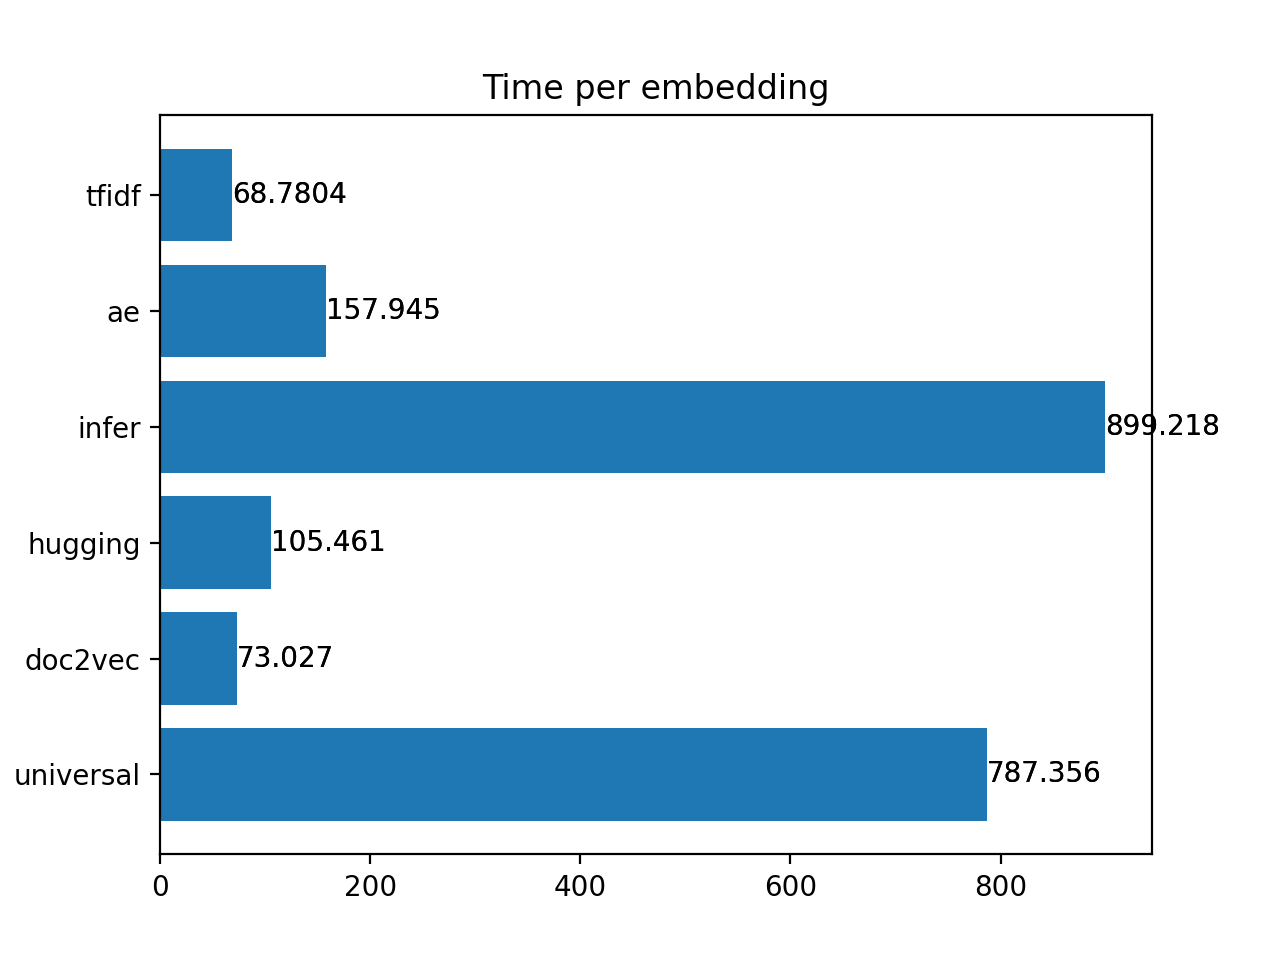
\includegraphics[width=5cm]{images/embeddings/infersent/time_per_doc_glove.png} }}%
    \qquad
    \subfloat[\centering Custom \ac{w2v} embeddings.]{{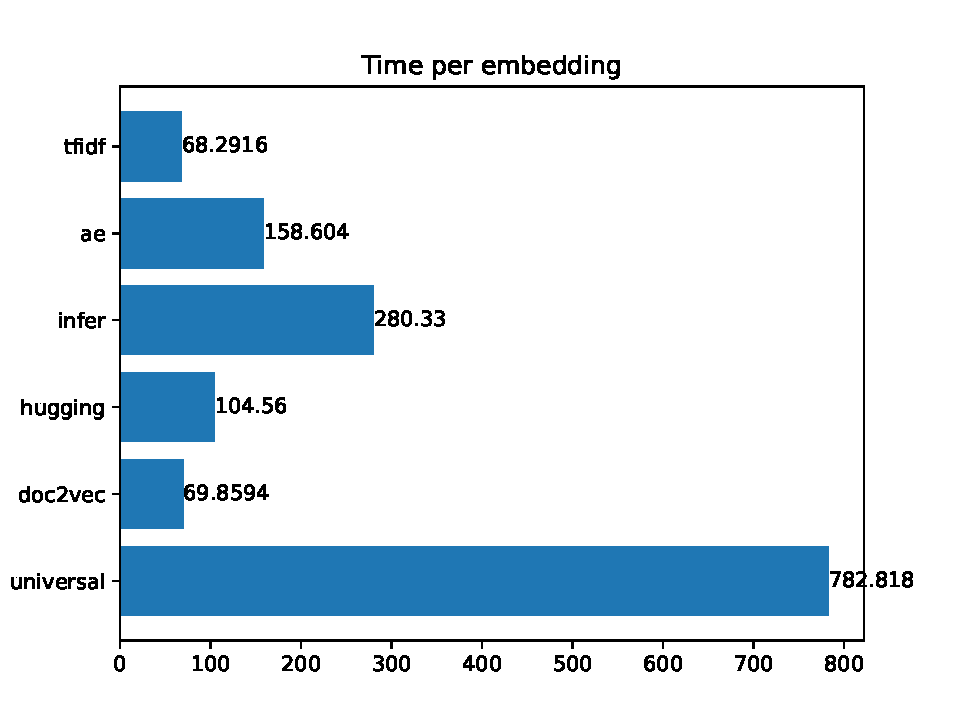
\includegraphics[width=5cm]{images/embeddings/infersent/time_per_doc_custom_emb.pdf} }}%
    \caption{Time (seconds) necessary to initialize the database, compute and insert 195 documents for specific embeddings.}%
    \label{fig:times_emb}%
\end{figure}






\section{analysis/ comparison of models}\label{sec:evaluation-models}
difference query responses for different models?
any images which produce unusual results?

\section{Evaluation of the performance}\label{sec:evaluation-performance}

\subsection{Fahnder clustern}\label{subsec:evaluation-metric1}

\subsection{Fahnder bewerten Resultate (image matrix)}\label{subsec:evaluation-metric2}

\section{Evaluation of the usability}\label{sec:evaluation-usability}

\subsection{Metrics}\label{subsec:evaluation-metrics}
    \chapter{Results}\label{ch:results}

Evaluate the results from the previous chapter.

\section{Fulfilment of objective}\label{sec:results-fulfilment}


\section{Research results}\label{sec:results-research}

    \chapter{Conclusion}\label{ch:conclusion}
    \chapter{Outlook}\label{ch:outlook}

\section{Future Work}\label{sec:future-work}


    % Die nächsten zwei Zeilen sind optional, sie sorgen dafür dass alles nach dem Inhalt wieder mit römischen Zahlen nummeriert wird.
    \pagenumbering{roman}
    \addtocounter{page}{4} % Dies ist die Anzahl der Seiten vor der Einleitung, muss möglicherweise angepasst werden, wenn das Inhaltsverzeichnis mehrere Seiten umfasst.

    \bibliography{
        bibliography/information-retrieval,
        bibliography/data-corpus,
        bibliography/embeddings,
        bibliography/database,
        bibliography/slurm,
        bibliography/clustering,
        bibliography/eigenfaces,
        bibliography/user_interface,
        bibliography/similarity,
        bibliography/autoencoder
    }

    \listoffigures
    \listoftables
    \renewcommand{\listoflistingscaption}{Listing-Verzeichnis}
    \listoflistings

    \appendix
    \chapter{Anhang}\label{ch:appendix}


    \chapter*{Declaration of authorship}

% Inhaltsverzeichnis und Kopfzeile
% \addcontentsline{toc}{chapter}{Eidesstattliche Erklärung}
\markboth{Declaration of authorship}{Declaration of authorship}

I hereby declare that I am the sole author of the bachelor’s thesis with the title "\thesistitle" 
and that I have not used any sources other than those listed in the bibliography and identified as references. 
I further declare that I have not submitted this thesis at any other institution in order to obtain a degree.

\vspace{1cm}

Kassel, \thesisdate

\begin{flushright}
  \underline{\hspace{7cm}} \\
  \thesisauthorname
\end{flushright}

\end{document}
